\documentclass[conference]{IEEEtran}
\IEEEoverridecommandlockouts
% The preceding line is only needed to identify funding in the first footnote. If that is unneeded, please comment it out.
%Template version as of 6/27/2024
\usepackage{placeins} % add to preamble — enables \FloatBarrier

\usepackage{cite}
\usepackage{amsmath,amssymb,amsfonts}
\usepackage{algorithmic}
\usepackage{graphicx}
\usepackage{textcomp}
\usepackage{xcolor}
\usepackage{tikz}
\usetikzlibrary{arrows.meta, positioning, fit, shadows, backgrounds}
\usepackage{url} % for \url command
\usepackage{booktabs} % for \toprule, \midrule, \bottomrule
\usetikzlibrary{shapes.geometric, arrows.meta, positioning}
\def\BibTeX{{\rm B\kern-.05em{\sc i\kern-.025em b}\kern-.08em
    T\kern-.1667em\lower.7ex\hbox{E}\kern-.125emX}}
\begin{document}

\title{TapLeak: Recovering WhatsApp Conversations via LLM-Augmented Acoustic Keystroke Inference}
% Acoustic Side-Channel Inference of Virtual Keyboard Input via Built-in Microphone}
% {\footnotesize \textsuperscript{*}Note: Sub-titles are not captured for https://ieeexplore.ieee.org  and
% should not be used}
% \thanks{Identify applicable funding agency here. If none, delete this.}
% }

% \author{\IEEEauthorblockN{1\textsuperscript{st} Given Name Surname}
% \IEEEauthorblockA{\textit{dept. name of organization (of Aff.)} \\
% \textit{name of organization (of Aff.)}\\
% City, Country \\
% email address or ORCID}
% \and
% \IEEEauthorblockN{2\textsuperscript{nd} Given Name Surname}
% \IEEEauthorblockA{\textit{dept. name of organization (of Aff.)} \\
% \textit{name of organization (of Aff.)}\\
% City, Country \\
% email address or ORCID}
% \and
% \IEEEauthorblockN{3\textsuperscript{rd} Given Name Surname}
% \IEEEauthorblockA{\textit{dept. name of organization (of Aff.)} \\
% \textit{name of organization (of Aff.)}\\
% City, Country \\
% email address or ORCID}
% \and
% \IEEEauthorblockN{4\textsuperscript{th} Given Name Surname}
% \IEEEauthorblockA{\textit{dept. name of organization (of Aff.)} \\
% \textit{name of organization (of Aff.)}\\
% City, Country \\
% email address or ORCID}
% \and
% \IEEEauthorblockN{5\textsuperscript{th} Given Name Surname}
% \IEEEauthorblockA{\textit{dept. name of organization (of Aff.)} \\
% \textit{name of organization (of Aff.)}\\
% City, Country \\
% email address or ORCID}
% \and
% \IEEEauthorblockN{6\textsuperscript{th} Given Name Surname}
% \IEEEauthorblockA{\textit{dept. name of organization (of Aff.)} \\
% \textit{name of organization (of Aff.)}\\
% City, Country \\
% email address or ORCID}
% }

\maketitle

% \begin{abstract}
% Billions of users daily entrust sensitive information
% %—private messages, passwords, and financial credentials—
% to virtual QWERTY keyboards on their smartphones while using applications such as WhatsApp, %Instagram, Facebook, 
% and mobile banking platforms. The security of this 
% % ubiquitous 
% input channel is implicitly assumed. Unlike physical keyboards, virtual keyboards produce no mechanical keystrokes, but they emit 
% % emitting 
% only faint acoustic signals
% % emanations 
% from the interaction of a fingertip with a glass surface. We tackle this assumption and demonstrate that these subtle sounds, captured by the built-in microphone of the device are sufficient to partially reconstruct the typed input, without any hardware modification and without knowledge of the user.
% %We present an end-to-end acoustic side-channel attack framework that exploits only microphone access, a permission routinely granted to messaging, social media, and utility applications on both Android and iOS. 
% In our attack model, the adversary can operate entirely within the normal permission model of a co-installed malicious app. We segment individual tap events from continuous audio via bandpass filtering and adaptive peak detection, extract a compact per-tap feature vector 
% % combining spectral kurtosis, fundamental pitch, and short-time energy, 
% and feed these into a neural classifier that produces a ranked top-5 candidate character set per keystroke. A two-stage text recovery module then prunes the candidate space: a trie-indexed dictionary search filters character sequences into valid English words, and a language model assigns perplexity-based scores to rank candidate sentences by linguistic plausibility.

% We evaluate our framework on a dataset spanning all 26 alphabetic characters 
% %recorded on a smartphone internal microphone. 
% While per-character top-1 classification is challenging,
% %— reflecting the acoustic similarity of touch events across a glass surface — 
% our top-5 candidate generation combined with trie-indexed dictionary filtering compresses the combinatorial search space by over 98\% accuracy. Also, a representative 4-character input yields 625 possible character sequences, of which only 7 are dictionary-valid English words. Language model perplexity re-ranking then identifies the most plausible sentence from this reduced candidate set. Our findings reveal that every session in which a user types on 
% %WhatsApp, Instagram, or 
% any application granted microphone permission is a potential eavesdropping surface. This highlights the need for acoustic-resilient virtual keyboard designs and tighter platform-level microphone access controls.


% We evaluate our framework on a dataset spanning all 26 alphabetic characters recorded on a smartphone internal microphone.While per-character top-1 classification remains challenging due to the acoustic similarity of touch events across the keyboard, our top-5 candidate generation combined with dictionary-constrained trie search and language model reranking successfully recovers plausible target words and sentences from ambiguous keystroke sequences — demonstrating that the attack is viable as a system even when individual character predictions are uncertain. Our findings reveal that every session in which a user types on WhatsApp, Instagram, or any application granted microphone permission is a potential eavesdropping surface, and motivate the need for acoustic-resilient virtual keyboard designs and tighter platform-level microphone access controls.
% Acoustic side-channel attacks have demonstrated that the sounds produced by physical keyboard keystrokes carry sufficient information to reconstruct typed text. Virtual QWERTY keyboards on touch-screen devices, however, present a qualitatively different challenge: they lack mechanical actuation, emitting only faint, position-dependent acoustic emanations from the interaction of a fingertip with a glass surface. Whether these subtle signals can be exploited for keystroke inference has received limited systematic investigation.

% We present an end-to-end framework for acoustic side-channel attacks on virtual touch-screen keyboards that requires only the device's built-in internal microphone—an adversary capability realizable by any application granted microphone permission. Our pipeline operates in four stages. First, we segment individual tap events from continuous audio using bandpass filtering and adaptive peak detection. Second, we extract a compact acoustic feature vector per tap combining spectral kurtosis, fundamental pitch, and short-time energy, which together capture the positional resonance signatures of glass-surface touch events. Third, a trained neural classifier generates a ranked top-k candidate character set for each tap. Finally, a two-stage text recovery module prunes the exponentially large candidate space: a trie-indexed dictionary search filters character sequences that form valid English words, and a language model assigns perplexity-based scores to rank candidate sentences by linguistic plausibility.

% We collect and evaluate a dataset spanning all 26 alphabetic characters on a smartphone internal microphone under realistic recording conditions. Our classifier achieves a test accuracy of 6.25\% under top-1 prediction—a 63\% relative improvement over the random baseline for a 26-class problem—and substantially higher recall under top-5 candidate generation. Our dictionary-plus-language-model recovery stage successfully reconstructs plausible target words from acoustically ambiguous per-character outputs. These results demonstrate the fundamental feasibility of acoustic eavesdropping on virtual keyboards and motivate the design of acoustic-resilient touch-screen input mechanisms.
% .\\ 
% .\\
% .\\
% .\\
% \begin{enumerate}

% \item Opening Context \& Problem Statement: smartphones, virtual keyboards, and security concerns.

% \item Specific Threat Introduction: ASCA in the context of virtual keyboards.

% \item High-Level Goal: States the main research question. (feasibility of retrieving typed words with ASCA)

% \item Method/Proposed Approach: the three technical points: ML, audio processing, NLP. [data collection (e.g., multiple devices, environments), feature extraction (MFCCs, spectrograms), and model (KNN, LLM).]

% \item Detailed Methodology: 1) Data Collection, 2) Segmentation, 3) Feature Extraction, 4) Classification (k-NN), 5) Word Reconstruction (Trie), 6) Sentence Scoring (LLM)

% \item Contribution Statement: Where is the work within existing literature? [Key Results]: top-10 character accuracy, generalizability across devices, robustness to noise.

% \item Practical Implication: [Real-world attack feasibility] This attack is feasible under realistic conditions (e.g., at a meeting or in a coffee shop). 

% \item Comparison (vs. physical keyboard attacks)

% \item Future Direction: Mitigation is needed. 
% \end{enumerate}
% \end{abstract}
\begin{abstract}
The widespread adoption of virtual QWERTY keyboards on smartphones has introduced a subtle yet serious security vulnerability: the acoustic emanations produced during typing. Applications such as WhatsApp, Instagram, Facebook, and banking platforms rely entirely on virtual keyboard input, and the sounds emitted while composing private messages, passwords, or financial transactions can be silently captured and decoded by a co-located device. In this paper, we present a complete end-to-end acoustic side-channel attack (ASCA) system that recovers typed text from the keystroke sounds of an iPhone~6 virtual keyboard recorded through the built-in microphone and the \textit{dB~Meter} iOS application. Our pipeline applies a 200--500\,Hz bandpass filter to isolate keystroke-relevant energy, extracts 14 acoustic features per keystroke segment, and employs Minimum Redundancy Maximum Relevance (MRMR) feature selection to identify the three most discriminative features---Spectral Kurtosis, Pitch, and Short-Time Energy. A $k$-Nearest Neighbour ($k$-NN, $k{=}10$) classifier achieves \textbf{100\% top-5 accuracy}, ensuring the correct character is always among the five most likely candidates. Candidate characters are then passed into a Trie constructed from the Google-10000-English corpus, which reduces the search space by \textbf{98.9\%} (from 625 to just 7 candidate words for a four-character target). A GPT-2 language model with perplexity-based reranking (threshold $< 100$) recovers the correct sentence consistently within the \textbf{top-3 predictions} for sentences up to twelve words, and as the \textbf{top-1 prediction} in controlled trials. These results demonstrate that virtual keyboard acoustics constitute a practical, low-cost eavesdropping vector requiring no hardware modifications, malware installation, or near field probing, posing a credible threat to user privacy on mobile messaging and financial platforms.
\end{abstract}
\begin{IEEEkeywords}
Acoustic side-channel attack · Virtual keyboard security · Keystroke inference · Trie-based word recovery · Smartphone microphone eavesdropping.
\end{IEEEkeywords}
\section{Introduction}
Every day, billions of people reach for their smartphones to send
a message, log in to their bank, or enter a password, and in
every one of those moments, the sole interface between the user
and the application is a virtual QWERTY keyboard drawn on a glass
screen. Instant messaging applications such as WhatsApp, Instagram, and Facebook
Messenger treat this keyboard as the
primary channel for sensitive input like private messages all pass through it. The security of this channel is taken for granted. Unlike a physical keyboard, which produces an audible mechanical click with every keypress, a touchscreen is silent in the conventional sense, no spring, no keycap, no typewriter
carriage. This silence is assumed to be privacy. We show that this assumption is wrong.

When a fingertip strikes a glass surface, it does not produce
silence. It produces a broadband acoustic impulse shaped by the
structural resonance of the device chassis, the position of the
tap on the screen, and the area of finger contact. These impulses
are faint, spectrally similar across different keys, and
superficially indistinguishable from background noise, but they
are not random. They carry positional information, and that
information can be extracted. This is the physical basis of an
\emph{acoustic side-channel attack} (ASCA) on a virtual keyboard:
an adversary who can record the sounds of a user typing can,
in principle, infer what was typed.

Acoustic side-channel attacks on \emph{physical} keyboards have
been studied since Asonov and Agrawal~\cite{asonov2004}
showed in 2004 that mechanical key sounds are sufficiently distinct
to enable character recovery from audio. Zhuang et
al.~\cite{zhuang2009keyboard} demonstrated that a language model
alone could correct a weak per-character classifier to achieve
practical word-level accuracy at several metres range.
Most recently, Harrison et al.~\cite{harrison2023deep} trained a deep convolutional network on smartphone microphone recordings of
a laptop keyboard and exceeded 93\% per-character top-1 accuracy,
establishing physical keyboard ASCA as a practical, deployable
threat. Virtual keyboards, however, have received far less systematic attention. They present a fundamentally different acoustic signature. There are no mechanical switches, no keycap resonators, and no typewriter carriages. The only acoustic event is the incidental sound produced when a fingertip contacts a rigid glass surface, a broadband impulse whose spectral properties vary subtly with the position of the tap on the screen, the structural resonances of the device chassis, and the contact area of the fingertip. These signals are quieter, more spectrally uniform across characters, and more sensitive to environmental noise than physical keyboard emissions. Crucially, this physical vulnerability is compounded by an underlying hardware-level flaw: electromagnetic (EM) crosstalk. Modern smartphones use high-density Flexible Printed Circuits (FPCs), with the touchscreen digitizer lines routed in close proximity to internal microphone traces. When a user interacts with the screen, the capacitive drive circuitry generates unique spatiotemporal EM emanations corresponding to the exact $(x, y)$ coordinate or targeted alphabet location. Because of insufficient internal shielding, these EM fluctuations are parasitically coupled directly into the microphone wiring, resulting in an immediate signal apprehension. 

A body of prior work has explored aspects of this problem without delivering a complete, end-to-end attack. Lu et al.~\cite{lu2019keylistener} proposed \textit{KeyListener}, a system that infers keystrokes on a QWERTY touch screen by exploiting acoustic signals captured by a microphone, demonstrating that position-dependent acoustic features can distinguish key regions on the screen in a controlled setting. The work by Md. F. Bari~\cite{ieee2021touch} further confirmed that acoustic emanations from touch interfaces carry recoverable input information, using machine learning to classify tap positions. \textit{Synesthesia}~\cite{genkin2019synesthesia} demonstrated an orthogonal threat, reconstructing displayed screen content from the acoustic emanations of LCD screens, illustrating the breadth of acoustic side channels in the modern device ecosystem. A recent review of keyboard acoustic attacks on Android devices~\cite{android2023} surveys the threat landscape in the context of digital banking, motivating the urgency of a rigorous attack evaluation on virtual keyboards.  \emph{Yet no prior study has closed the loop from raw microphone audio to recovered English
text for arbitrary alphabetic input.} The gap is not merely empirical, it reflects a fundamental difference in the problem structure: virtual keyboard tap sounds are weaker, more uniform across the key space, and require a different strategy than the
feature-classifier pipelines that dominate physical keyboard attacks. So here is a pertinent question that we try to answer in this paper:
\\
\noindent\textit{Can an attacker armed with nothing but access to the internal microphone reconstruct words and sentences typed on a smartphone
touchscreen, without touching the device, without exploiting
any software vulnerability, and without the user's knowledge?}

\emph{We present a complete, end-to-end ASCA pipeline for virtual touch-screen keyboards.} The attacker controls only the victim device's built-in microphone,
accessible to any co-installed application granted standard microphone
permission---a permission held by a large fraction of popular messaging,
social media, and utility applications on both Android and iOS. The
attacker has no access to the screen, no inertial sensor data, no network
traffic, and no knowledge of which application is in use. During any
session in which the victim types on their virtual keyboard, the attacker
passively records audio and processes it offline to recover the typed text.
No user-specific enrollment is required.

This paper makes the following contributions:

\begin{itemize}

  \item \textbf{End-to-end virtual keyboard ASCA pipeline.}
  We present the first complete acoustic side-channel attack on a virtual
  QWERTY keyboard requiring only standard microphone permission. Starting
  from raw audio, a Butterworth bandpass filter (200--500\,Hz) and adaptive
  peak detection isolate individual tap events. Each tap is represented by
  a compact feature vector comprising MFCCs, Harmonics-to-Noise Ratio,
  Spectral Centroid, and Zero Crossing Rate, capturing both the
  glass-surface impact acoustics and electromagnetic emission artifacts
  induced in the microphone circuit by the screen's electrode matrix
  \cite{EMnAcoustic2026}. A $k$-NN classifier trained on these features
  returns a ranked top-5 candidate character set per keystroke rather than
  a single hard prediction, deliberately propagating acoustic uncertainty
  into the downstream recovery stage.

  \item \textbf{Trie and LLM recovery stage.}
  We show that trie-based dictionary filtering reduces the $5^n$
  character-combination search space by over 98\% for typical English word
  lengths---compressing 625 combinations to 7 candidates for a
  representative 4-character input---without discarding the correct target.
  GPT-2 perplexity re-ranking over the surviving word hypotheses
  consistently places the correct sentence in the top-3 predictions, and
  at the top-1 position in controlled trials, demonstrating that lexical
  and linguistic constraints reliably compensate for weak per-character
  acoustic classification.

  \item \textbf{Evaluation and mitigation.}
  We evaluate the full pipeline on a 26-character smartphone tap dataset,
  achieving 100\% top-5 character accuracy---the correct character is
  always present in the classifier's top-5 candidates. Confusion matrix
  analysis reveals that residual errors are dominated by acoustically
  adjacent keys rather than random misclassification, confirming that the
  attack's failure modes are structured and predictable. Building on these
  observations, we discuss concrete countermeasures---microphone gating,
  acoustic masking, and keyboard layout randomization---and assess their
  effectiveness against the specific confusions the system exhibits.

\end{itemize}

% The attacker controls the victim device's own built-in microphone, that is accessible to any co-installed application granted standard microphone permission. This permission is held by a large fraction of popular messaging, social media, and utility applications on both Android and iOS. The attacker has no access to the screen, no inertial sensor data, no network traffic, and no knowledge of which application is in use. During any session in which the victim types on their virtual keyboard, the attacker passively records audio and processes it offline to recover the typed text. No user-specific enrollment is required. Starting from raw audio, our system uses Butterworth bandpass filtering and adaptive peak detection to find tap events. It then extracts a compact acoustic feature vector for each tap. This includes Mel-Frequency Cepstral Coefficients (MFCCs), Harmonics-to-Noise Ratio (HNR), Spectral Centroid, and Zero Crossing Rate. These features capture the tonal and noise-like parts of a glass-surface impact. They also capture artifacts from EM emissions in the screen matrix wires, which are detected by the microphone and affect its wiring \cite{EMnAcoustic2026}. A $k$-nearest neighbour ($k$-NN) classifier, trained on these features, produces a ranked top-5 candidate character set for each tap rather than a single hard prediction, propagating acoustic uncertainty into the downstream recovery stage. A trie-indexed English dictionary search then filters the $5^n$ possible character strings to dictionary-valid words, compressing a 625-combination search space for a representative
% 4-character input to just 7 candidate words, a reduction of over 98\%, without discarding the correct target. Finally, GPT-2 perplexity scoring ranks the surviving candidates by linguistic plausibility and returns the most natural sentence hypothesis. This cascade of constraints, acoustic classification, lexical
% filtering, and language model re-ranking, allows the system to recover typed words reliably even when individual character
% predictions are uncertain.
% \subsection*{Contributions}

% This paper makes the following contributions:

% \begin{itemize}

%   \item \textbf{End-to-end virtual keyboard ASCA pipeline.}
%   We present the first complete acoustic side-channel attack on a
%   virtual QWERTY keyboard that requires only standard microphone
%   permission, producing recovered English text from raw audio
%   via a k-NN, Trie and Large Language Model (LLM) architecture.

%   \item \textbf{Trie and LLM recovery stage.}
%   We show that trie-based dictionary filtering compresses a
%   $5^n$ character-combination space by over 98\% for typical
%   word lengths, and that GPT-2 perplexity re-ranking selects the
%   correct word from the surviving candidates; demonstrating that
%   linguistic constraints compensate for weak per-character
%   acoustic classification.

%   \item \textbf{Evaluation and mitigation.}
%   We evaluate the full pipeline on a 26-character smartphone
%   tap dataset and discuss concrete countermeasures, microphone
%   gating, acoustic masking, and keyboard layout
%   randomization, grounded in the attack's observed failure modes.

% \end{itemize}

The remainder of the paper is organised as follows. Section~\ref{sec:background} reviews related work. Section~\ref{sec:model} explains the threat model. Section~\ref{sec:methodology} describes the system design. Section~\ref{sec:results} presents experimental results. Section~\ref{sec:discussion} discusses limitations and mitigations. Section~\ref{sec:conclusion} concludes.


% \section{Background \& Related Work}

% \subsection{Acoustic Side-Channel Attacks on Physical Keyboards}

% \textbf{Classic work.}
% The vulnerability of physical keyboards to acoustic eavesdropping was
% first demonstrated by Asonov and Agrawal~\cite{asonov2004}, who showed
% in 2004 that the mechanical sound produced by each keycap is
% sufficiently distinctive to allow character recovery from audio
% recordings captured at close range.
% The core observation is that each key sits atop a different spring
% mechanism and acts as a resonator of slightly different geometry,
% imprinting a unique spectral fingerprint on the emitted impulse.
% Zhuang~et~al.~\cite{zhuang2005} later showed that this attack can be
% mounted without any labeled training data: by clustering unlabeled
% keystroke recordings and coupling the resulting soft labels to a
% statistical English dictionary, they achieved word-level recovery
% accuracies of up to 73\% from recordings made several metres away.
% Their work established the critical role of \emph{linguistic
% priors}---the observation that even a weak per-character classifier
% can be corrected to a high degree by constraining its output to
% plausible word sequences.

% \textbf{Feature extraction.}
% Early acoustic keyboard attacks relied on time-domain features such
% as peak amplitude and inter-keystroke intervals, but subsequent work
% demonstrated that frequency-domain representations carry richer
% discriminative information.
% Mel-frequency cepstral coefficients (MFCCs), originally developed for
% speech recognition, capture the coarse spectral envelope of a
% keystroke impulse and have become the de-facto feature for acoustic
% side-channel classification~\cite{zhuang2005,harrison2023}.
% Short-time Fourier transform (STFT) spectrograms preserve finer
% temporal-spectral structure and have been used as input to
% convolutional neural networks that learn task-specific features
% directly from the two-dimensional representation.

% \textbf{Classifiers.}
% The classifier landscape has evolved in step with feature
% representations.
% Early work used $k$-nearest neighbours (k-NN) and Hidden Markov
% Models (HMMs), both of which pair naturally with MFCC vectors.
% HMMs are particularly attractive because they model the temporal
% dynamics of a keystroke sequence, enabling joint character-sequence
% decoding that implicitly incorporates language constraints.
% Harrison~et~al.~\cite{harrison2023} replaced HMMs with a
% CoAtNet~\cite{dai2021coatnet}---a convolutional-transformer hybrid
% that treats STFT spectrograms as images---and achieved a top-1
% per-character accuracy of 93\% on laptop keyboard audio recorded
% by a co-located smartphone microphone, and 95\% on audio captured
% by a Zoom meeting microphone.
% This result demonstrates that deep learning has made physical
% keyboard acoustic attacks not merely feasible but practically
% devastating, motivating the need to understand whether the same
% threat extends to virtual keyboards.

% % -------------------------------------------------------------------

% \begin{table*}[t]
% \centering
% \caption{Comparison of acoustic side-channel attacks on keyboards.
%          \checkmark~=~present; \texttimes~=~absent; 
%          N/R~=~not reported at character level.}
% \label{tab:related}
% \renewcommand{\arraystretch}{1.25}

% \begin{tabular}{lccccccc}
% \hline
% \textbf{Work} &
% \textbf{Keyboard} &
% \textbf{Mic} &
% \textbf{Classifier} &
% \textbf{Trie} &
% \textbf{LLM} &
% \textbf{Granularity} &
% \textbf{End-to-End} \\
% \hline
% Asonov \& Agrawal~\cite{asonov2004}
%   & Physical & External & Neural Net  & \texttimes & \texttimes & Character  & \texttimes \\
% Zhuang et al.~\cite{zhuang2005}
%   & Physical & External & k-NN + HMM  & \checkmark & \texttimes & Word       & Partial \\
% Harrison et al.~\cite{harrison2023}
%   & Physical & Smartphone & CoAtNet   & \texttimes & \texttimes & Character  & Partial \\
% Lu et al.~\cite{lu2019keylistener}
%   & Virtual  & External & SVM         & \texttimes & \texttimes & Region     & \texttimes \\
% \cite{retrieving2021} DSC~2021
%   & Virtual  & External & ML          & \texttimes & \texttimes & Tap pos.   & \texttimes \\
% \hline
% \textbf{This work}
%   & \textbf{Virtual} & \textbf{Internal} & \textbf{k-NN}
%   & \checkmark & \checkmark
%   & \textbf{Word / Sentence} & \checkmark \\
% \hline
% \end{tabular}



% % \begin{tabular}{lcccccccc}
% % \hline
% % \textbf{Work} &
% % \textbf{Keyboard} &
% % \textbf{Microphone} &
% % \textbf{Classifier} &
% % \textbf{Top-1 Acc.} &
% % \textbf{Dictionary/} &
% % \textbf{LLM} &
% % \textbf{End-to-End} \\
% % & \textbf{Type} & \textbf{Type} & & & \textbf{Trie} & \textbf{Reranking} &
% % \textbf{Text Recovery} \\
% % \hline
% % Asonov \& Agrawal~\cite{asonov2004}
% %   & Physical & External & Neural Net   & $\sim$80\%  & \texttimes & \texttimes & \texttimes \\
% % Zhuang et al.~\cite{zhuang2005}
% %   & Physical & External & k-NN + HMM   & $\sim$73\%$^\dagger$  & \checkmark & \texttimes & Partial \\
% % Harrison et al.~\cite{harrison2023}
% %   & Physical & Smartphone & CoAtNet (DL) & 93--95\% & \texttimes & \texttimes & Partial \\
% % Lu et al.~\cite{lu2019keylistener}
% %   & Virtual  & External & SVM          & N/R (region) & \texttimes & \texttimes & \texttimes \\
% % \cite{retrieving2021} (DSC 2021)
% %   & Virtual  & External & ML           & N/R (limited vocab.) & \texttimes & \texttimes & \texttimes \\
% % \hline
% % \textbf{This work}
% %   & \textbf{Virtual} & \textbf{Internal} & \textbf{k-NN}
% %   & \textbf{6.25\%}
% %   & \checkmark & \checkmark & \checkmark \\
% % \hline
% % \end{tabular}
% \smallskip\\
% \raggedright
% \small{$^\dagger$ Reported at word level after dictionary correction, not per-character top-1.}
% \end{table*}


% \subsection{Virtual Keyboards and Their Acoustics}

% \textbf{Acoustic physics of capacitive touchscreens.}
% A capacitive touchscreen has no mechanical switch beneath each
% ``key'': the entire keyboard occupies a uniform glass surface whose
% actuation is detected by changes in capacitance at a touch-sensing
% grid.
% When a fingertip contacts the glass, it produces a broadband
% acoustic impulse that arises from at least four physical
% mechanisms:
% (i)~the \emph{impact sound} of soft tissue striking a rigid
% glass–metal sandwich;
% (ii)~\emph{structural vibrations} of the glass panel and device
% chassis, whose resonance modes depend on the position of the tap
% relative to the chassis geometry;
% (iii)~\emph{sliding friction} if the finger is dragged before
% lifting; and
% (iv)~\emph{electromagnetic coupling} of the voltage transitions on
% the touch-sensing wire grid into the device's microphone circuitry
% via the shared ground plane.
% The net signal reaching the internal microphone is therefore a
% superposition of all four components.
% Crucially, the structural resonance contribution (ii) makes the
% received waveform position-dependent: taps near the centre of the
% screen excite different chassis modes than taps near the edges, and
% taps on the left half of the keyboard excite a subtly different
% impulse response than taps on the right half.
% This position dependence is the physical basis on which any acoustic
% side-channel attack on a virtual keyboard must rely.

% \textbf{Prior work on tap inference.}
% Lu~et~al.~\cite{lu2019keylistener} proposed KeyListener, which
% captures acoustic signals from a QWERTY touch-screen keyboard and
% uses them to infer keystrokes.
% Their system segments individual taps from continuous audio,
% extracts acoustic features, and applies a machine-learning classifier
% that distinguishes broad key \emph{regions} (left vs.\ right half,
% upper vs.\ lower row) with reasonable accuracy in a controlled
% laboratory setting.
% A subsequent study~\cite{retrieving2021} confirmed at IEEE DSC~2021
% that acoustic emanations from touch interfaces contain recoverable
% per-tap information when machine-learning classifiers are applied to
% short-time spectral features, reporting positive results on a
% constrained key vocabulary.
% A recent survey of keyboard acoustic attacks targeting Android
% devices in the context of digital
% banking~\cite{android2023} catalogues the growing
% threat landscape and calls for rigorous evaluation of virtual
% keyboard eavesdropping.
% Orthogonal work by Genkin~et~al.~\cite{genkin2019synesthesia} showed
% that the acoustic emanations of LCD screens can reveal the
% \emph{content displayed} on the screen, a different threat vector
% that nonetheless reinforces the general principle that modern
% consumer devices leak acoustic information in non-obvious ways.
% Despite this body of evidence, no prior work has demonstrated a
% complete, deployable pipeline that takes raw audio from a device's
% internal microphone and produces recovered English text for arbitrary
% alphabetic input---the gap our work fills.

% % -------------------------------------------------------------------
% \subsection{Language Models in Side-Channel Attacks}

% \textbf{Dictionary and trie filtering.}
% Incorporating lexical knowledge to improve the output of a
% character-level acoustic classifier was first formalised by
% Zhuang~et~al.~\cite{zhuang2005}, who used a pre-built English
% dictionary to rule out impossible character sequences, reducing the
% effective search space from an exponential combinatorial problem to a
% manageable set of plausible words.
% Subsequent keylogging research has standardised this idea: given the
% top-$k$ candidate characters at each keystroke position, one
% enumerates all length-consistent strings that appear in the
% dictionary.
% A \emph{trie} (prefix tree) is the canonical data structure for this
% step, because it prunes impossible paths early during depth-first
% search, allowing the full dictionary to be traversed without
% materialising all $k^{n}$ candidate strings
% explicitly~\cite{zhuang2005}.
% In our system, a trie indexed over a 370,000-word English lexicon
% reduces a 4-character, top-5-per-position search space from 625
% candidate strings to a handful of dictionary-valid words---a
% compression of over 98\%---before any linguistic scoring is applied.


% \textbf{Language models for sentence reconstruction.}
% Once candidate words are identified, reconstructing the most
% plausible multi-word sentence is a natural language understanding
% problem.
% Statistical $n$-gram language models have been used to rescore
% candidate sequences in classical acoustic keyboard attacks, but
% their coverage is limited by corpus size.
% Large pre-trained neural language models, such as
% GPT-2~\cite{radford2019gpt2}, compute \emph{perplexity}---the
% inverse probability a model assigns to a token sequence---as a
% continuous, finely calibrated plausibility score.
% To the best of our knowledge, the use of a pre-trained large
% language model for perplexity-based candidate reranking in an
% acoustic side-channel attack is novel.
% Our pipeline scores every candidate word sequence recovered by the
% trie filter using GPT-2 perplexity and returns the sequence with the
% lowest perplexity as the attack's sentence hypothesis, combining
% lexical feasibility with contextual naturalness in a single
% end-to-end recovery stage.

% Table~\ref{tab:related} summarises the comparison.
% As the table shows, no prior work targets a virtual keyboard
% with an internal microphone, uses both a trie and a language
% model, and delivers end-to-end text recovery---the combination
% that defines the contribution of this paper.



% -------------------------------------------------------------------

\section{Background \& Related Work} \label{sec:background}
This section discusses the related studies and emphasizes the gap covered in our work.
\begin{table*}[!ht]
\centering
\caption{Comparison of representative acoustic and sensor side-channel attacks on keyboard input}
\label{tab:comparison}
\renewcommand{\arraystretch}{1.2}
\begin{tabular}{lllllll}
\toprule
\textbf{Work} & \textbf{Target} & \textbf{Sensor} & \textbf{Setup} & \textbf{ML Method} & \textbf{Output Granularity} & \textbf{LLM Post-proc.} \\
\midrule
Asonov \& Agrawal~\cite{asonov2004}   & Desktop keyboard  & Microphone   & Lab       & Neural Network      & Character          & No  \\
Zhuang et al.~\cite{zhuang2009keyboard}        & Desktop keyboard  & Microphone   & Lab       & SVM + HMM           & Word               & HMM \\
KeyListener~\cite{lu2019keylistener}           & Android virtual KB & Accel./Gyro & Co-located & SVM                & Character          & No  \\
Synesthesia~\cite{genkin2019synesthesia}       & LCD screen        & EM sensor    & Proximate  & Template match      & Screen content     & No  \\
Harrison et al.~\cite{harrison2023deep}            & Laptop keyboard   & Smartphone mic & Co-located & CNN               & Character          & GPT-2 \\
Retrieving~\cite{ieee2021touch}              & Physical keyboard  & Microphone   & Remote     & CNN                & Word               & LM  \\
\textbf{This work}                             & \textbf{iPhone virtual KB} & \textbf{Smartphone mic} & \textbf{Co-located} & \textbf{$k$-NN + MRMR} & \textbf{Sentence} & \textbf{GPT-2} \\
\bottomrule
\end{tabular}
\end{table*}
% \begin{table*}[!ht]
% \centering
% \caption{Comparison of acoustic side-channel attacks on keyboards.
%          \checkmark~=~present; \texttimes~=~absent.}
% \label{tab:related}
% \renewcommand{\arraystretch}{1.25}
% \begin{tabular}{lccccccc}
% \hline
% \textbf{Work} &
% \textbf{Keyboard} &
% \textbf{Mic} &
% \textbf{Classifier} &
% \textbf{Trie} &
% \textbf{LLM} &
% \textbf{Granularity} &
% \textbf{End-to-End} \\
% \hline
% Asonov \& Agrawal~\cite{asonov2004}
%   & Physical & External & Neural Net   & \texttimes & \texttimes & Character        & \texttimes \\
% Zhuang et al.~\cite{zhuang2005}
%   & Physical & External & k-NN + HMM   & \checkmark & \texttimes & Word             & Partial    \\
% Harrison et al.~\cite{harrison2023}
%   & Physical & Smartphone & CoAtNet    & \texttimes & \texttimes & Character        & Partial    \\
% Lu et al.~\cite{lu2019keylistener}
%   & Virtual  & External & SVM          & \texttimes & \texttimes & Region           & \texttimes \\
% \cite{retrieving2021} DSC~2021
%   & Virtual  & External & ML           & \texttimes & \texttimes & Tap position     & \texttimes \\
% \hline
% \textbf{This work}
%   & \textbf{Virtual} & \textbf{Internal} & \textbf{k-NN}
%   & \checkmark & \checkmark & \textbf{Word / Sentence} & \checkmark \\
% \hline
% \end{tabular}
% \end{table*}
\subsection{Acoustic Side-Channel Attacks on Physical Keyboards}

\textbf{Classic work.}
The vulnerability of physical keyboards to acoustic eavesdropping was first demonstrated by Asonov and Agrawal~\cite{asonov2004}, who showed in 2004 that the mechanical sound produced by each keycap is
sufficiently distinctive to allow character recovery from audio
recordings captured at close range.
The core observation is that each key sits atop a different spring
mechanism and acts as a resonator of slightly different geometry,
imprinting a unique spectral fingerprint on the emitted impulse.
Zhuang~et~al.~\cite{zhuang2005} later showed that this attack can be
mounted without any labelled training data: by clustering unlabelled keystroke recordings and coupling the resulting soft labels to a statistical English dictionary, they achieved word-level recovery accuracies of up to 73\% from recordings made several metres away. Their work established the critical role of \emph{linguistic
priors}; the observation that even a weak per-character classifier
can be corrected to a high degree by constraining its output to
plausible word sequences.

\textbf{Feature extraction.}
Early acoustic keyboard attacks relied on time-domain features such
as peak amplitude and inter-keystroke intervals, but subsequent work demonstrated that frequency-domain representations carry richer
discriminative information.
Mel-frequency cepstral coefficients (MFCCs), originally developed for
speech recognition, capture the coarse spectral envelope of a
keystroke impulse and have become the de-facto feature for acoustic
side-channel classification~\cite{zhuang2005,harrison2023}.
Short-time Fourier transform (STFT) spectrograms preserve finer
temporal-spectral structure and have been used as input to
convolutional neural networks that learn task-specific features
directly from the two-dimensional representation.

\textbf{Classifiers.}
The classifier landscape has evolved in step with feature representations.
Early work used k-NN and Hidden Markov Models (HMMs), both of which pair naturally with MFCC vectors.
HMMs are particularly attractive because they model the temporal
dynamics of a keystroke sequence, enabling joint character-sequence
decoding that implicitly incorporates language constraints.
Harrison~et~al.~\cite{harrison2023deep} replaced HMMs with a
CoAtNet~\cite{dai2021coatnet}; a convolutional-transformer hybrid model that treats STFT spectrograms as images. Their model achieved a top-1 per-character accuracy of 93\% on laptop keyboard audio recorded by a co-located smartphone microphone, and 95\% on audio captured by a Zoom meeting microphone.
This result demonstrates that deep learning has made physical
keyboard acoustic attacks not merely feasible but practically
devastating, motivating the need to understand whether the same
threat extends to virtual keyboards.

% -------------------------------------------------------------------
% \subsection{Virtual Keyboards and Their Acoustics}

% \textbf{Acoustic physics of capacitive touchscreens.}
% A capacitive touchscreen has no mechanical switch beneath each
% ``key'': the entire keyboard occupies a uniform glass surface whose actuation is detected by changes in capacitance at a touch-sensing grid.
% When a fingertip contacts the glass, it produces a broadband
% acoustic impulse that arises from at least four physical mechanisms:
% (i)~the \emph{impact sound} of soft tissue striking a rigid
% glass-metal sandwich;
% (ii)~\emph{structural vibrations} of the glass panel and device
% chassis, whose resonance modes depend on the position of the tap
% relative to the chassis geometry;
% (iii)~\emph{sliding friction} if the finger is dragged before
% lifting; and
% (iv)~\emph{electromagnetic coupling} of the voltage transitions on the touch-sensing wire grid into the device's microphone circuitry via the shared ground plane.
% Crucially, the structural resonance contribution~(ii) makes the
% received waveform position-dependent: taps near the center of the screen excite different chassis modes than taps near the edges, and
% taps on the left half of the keyboard excite a subtly different
% impulse response than taps on the right half.
% This position dependence is the physical basis on which any acoustic
% side-channel attack on a virtual keyboard must rely.

% \textbf{Prior work on tap inference.}
% Lu~et~al.~\cite{lu2019keylistener} proposed KeyListener, which
% captures acoustic signals from a QWERTY touch-screen keyboard and
% uses them to infer keystrokes.
% Their system segments individual taps from continuous audio,
% extracts acoustic features, and applies a machine-learning classifier that distinguishes broad key \emph{regions} (left vs.\ right half, upper vs.\ lower row) with reasonable accuracy in a controlled
% laboratory setting.
% A subsequent study~\cite{retrieving2021} confirmed at IEEE DSC~2021
% that acoustic emanations from touch interfaces contain recoverable
% per-tap information when machine-learning classifiers are applied to
% short-time spectral features, reporting positive results on a
% constrained key vocabulary.
% A recent survey of keyboard acoustic attacks targeting Android
% devices in the context of digital banking~\cite{android2023}
% catalogs the growing threat landscape and calls for rigorous
% evaluation of virtual keyboard eavesdropping.
% Orthogonal work by Genkin~et~al.~\cite{genkin2019synesthesia} showed
%  hat the acoustic emanations of LCD screens can reveal the \emph{content displayed} on the screen, reinforcing the general principle that modern consumer devices leak acoustic information in non-obvious ways.

% \textbf{Our work}, ``TapLeak" exploits a hybrid hardware vulnerability: the localized acoustic impulse from a screen tap, combined with simultaneous EM crosstalk from the touchscreen matrix wires into adjacent, unshielded internal microphone wiring. 


\subsection{Virtual Keyboards and Their Acoustics}

\textbf{Acoustic physics of capacitive touchscreens.}
A capacitive touchscreen has no mechanical switch beneath each
``key'': the entire keyboard occupies a uniform glass surface whose
actuation is detected by changes in capacitance at a touch-sensing grid.
When a fingertip contacts the glass, it produces a broadband
acoustic impulse that arises from at least four physical mechanisms:
(i)~the \emph{impact sound} of soft tissue striking a rigid
glass-metal sandwich;
(ii)~\emph{structural vibrations} of the glass panel and device
chassis, whose resonance modes depend on the position of the tap
relative to the chassis geometry;
(iii)~\emph{sliding friction} if the finger is dragged before
lifting; and
(iv)~\emph{electromagnetic coupling} of the voltage transitions on
the touch-sensing wire grid into the device's microphone circuitry
via the shared ground plane~\cite{EMnAcoustic2026}, a hardware
crosstalk path that has been independently confirmed on commodity
smartphones. The opened iPhone~6 in Figure~\ref{fig:iPhone6Wires} shows the wires of the screen, and illustrates that they are close to the front microphone of the device; the golden colored element shown in Figure~\ref{fig:iphone6Mic}.
Crucially, the structural resonance contribution~(ii) makes the
received waveform position-dependent: taps near the center of the
screen excite different chassis modes than taps near the edges, and
taps on the left half of the keyboard excite a subtly different
impulse response than taps on the right half.
This position dependence is the physical basis on which any acoustic
side-channel attack on a virtual keyboard must rely.
\begin{figure}[htbp]
    \centering
    % Left Image
    \begin{minipage}[b]{0.48\linewidth}
        \centering
        \includegraphics[width=\linewidth]{figures/wiresofscreenconv2.jpg}
        \caption{Wires of the touch screen above the front microphone of iPhone~6.}
        \label{fig:iPhone6Wires}
    \end{minipage}
    \hfill % Pushes the images to the left and right edges
    % Right Image
    \begin{minipage}[b]{0.48\linewidth}
        \centering
        \includegraphics[width=1.1\linewidth, angle=90]{figures/micOntopconv.jpg}
        \caption{Microphone positioned on top of iPhone~6.}
        \label{fig:iphone6Mic}
    \end{minipage}
\end{figure}

\textbf{Prior work on tap inference.}
Lu~et~al.~\cite{lu2019keylistener} proposed KeyListener, which
captures acoustic signals from a QWERTY touch-screen keyboard and
uses them to infer keystrokes.
Their system segments individual taps from continuous audio,
extracts acoustic features, and applies a machine-learning classifier
that distinguishes broad key \emph{regions} (left vs.\ right half,
upper vs.\ lower row) with reasonable accuracy in a controlled
laboratory setting.
A subsequent study~\cite{ieee2021touch} confirmed at IEEE DSC~2021
that acoustic emanations from touch interfaces contain recoverable
per-tap information when machine-learning classifiers are applied to
short-time spectral features, reporting positive results on a
constrained key vocabulary.
A recent survey of keyboard acoustic attacks targeting Android
devices in the context of digital banking~\cite{android2023}
catalogs the growing threat landscape and calls for rigorous
evaluation of virtual keyboard eavesdropping.
Orthogonal work by Genkin~et~al.~\cite{genkin2019synesthesia} showed
that the acoustic emanations of LCD screens can reveal the
\emph{content displayed} on the screen, reinforcing the general
principle that modern consumer devices leak acoustic information in
non-obvious ways.

\textbf{Our work.}
TapLeak advances beyond region-level inference to full per-character
recovery. We extract a compact feature vector per tap comprising
MFCCs, Harmonics-to-Noise Ratio, Spectral Centroid, and Zero
Crossing Rate that captures all four physical mechanisms described
above, and train a $k$-NN classifier to produce a ranked top-5
candidate character set per keystroke rather than a single hard
prediction. A trie-indexed dictionary search then prunes the $5^n$ combination space by over 98\%, and GPT-2 perplexity scoring
re-ranks the surviving word hypotheses by linguistic plausibility. The result is a pipeline that recovers full typed sentences from raw audio, using only the microphone permission already held by a wide class of installed applications, and without any user-specific enrollment.

% -------------------------------------------------------------------
\subsection{Language Models in Side-Channel Attacks}

\textbf{Dictionary and trie filtering.}
Incorporating lexical knowledge to improve the output of a character-level acoustic classifier was first formalized by Zhuang~et~al.~\cite{zhuang2005}, who used a pre-built English dictionary to rule out impossible character sequences, reducing the
effective search space from an exponential combinatorial problem to a manageable set of plausible words. Subsequent key-logging research has standardized this idea: given the top-$k$ candidate characters at each keystroke position, one enumerates all length-consistent strings that appear in the dictionary.
A \emph{trie} (prefix tree) is the canonical data structure for this
step, because it prunes impossible paths early during depth-first
search, allowing the full dictionary to be traversed without
materializing all $k^{n}$ candidate strings explicitly~\cite{zhuang2005}.

\textbf{Language models for sentence reconstruction.}
Once candidate words are identified, reconstructing the most
plausible multi-word sentence is a natural language understanding
problem. Statistical $n$-gram language models have been used to rescore candidate sequences in classical acoustic keyboard attacks, but their coverage is limited by corpus size.
Large pre-trained neural language models, such as GPT-2~\cite{radford2019gpt2}, compute \emph{perplexity}; the
inverse probability a model assigns to a token sequence, as a
continuous, finely calibrated plausibility score.
To the best of our knowledge, applying a pre-trained large language model for perplexity-based candidate re-ranking in an acoustic
side-channel attack is novel in this work.

% -------------------------------------------------------------------
% TABLE PLACED HERE — after all three subsections have been introduced
% \FloatBarrier forces LaTeX to place the table before starting
% the next section


As Table~\ref{tab:comparison} shows, no prior work targets a virtual
keyboard using an internal microphone, combines a trie with a
language model, and delivers end-to-end text recovery, the
combination that defines the contribution of this paper.



\section{Threat Model}\label{sec:model}

We now formalize the adversary and victim assumptions under which
our attack operates.

\textbf{Adversary capabilities.}
The attacker controls the victim device's own built-in microphone,
accessed through a co-installed malicious application that holds
standard microphone permission. This permission is granted routinely to messaging, social media, and utility applications on both Android and iOS~\cite{android2023}. 
Critically, this permission model does not restrict \emph{when}
microphone access is permitted: an application holding it can
record audio at any time, including while the user is typing in an
entirely different application.
In our implementation, audio is captured using a commercial
sound-level meter application (dB Meter), shown in Figure~\ref{fig:dbmeter}, which records continuous audio for measuring ambient noise levels.
This represents a realistic and practically undetectable attack
vector: a dB meter application is a plausible, benign-looking app
that users would not associate with keystroke eavesdropping, yet it
provides the attacker with a continuous, high-quality audio stream from the internal microphone.
There is no access to the device's accelerometer, gyroscope,
camera, or any other sensor, and there is no visibility of the
screen content or the application being used.
The attacker does not need physical contact with the device, does
not require any user-specific enrollment or calibration session,
and operates entirely passively during the attack phase.

\begin{figure}[!ht]
  \centering
  \includegraphics[width=0.45\linewidth]{figures/dbmeter_screenshot.png}
  \caption{The dB Meter application used for audio capture in this
           study. The app records continuous audio under the guise
           of measuring ambient sound levels, requiring only
           standard microphone permission on Android/iOS.}
  \label{fig:dbmeter}
\end{figure}

\textbf{Victim behavior.}
The victim types on a standard QWERTY virtual keyboard displayed on
a touch-screen smartphone.
The attack is evaluated on the 26-character \emph{alphabetic}
keyspace (a-z); digits, punctuation, and special characters are outside the current scope.
The victim may be typing in any application that uses the system
virtual keyboard, including messaging platforms (WhatsApp, Instagram, or Facebook Messenger), password fields, note-taking apps, and mobile banking interfaces.
No specific application, network connection, or operating system
version is assumed.

\textbf{Attacker goal.}
Given the audio recording of a typing session, the attacker recovers the sequence of words typed by the victim.
Success is measured at the \emph{word level}: the attack is
considered successful if the correct target word appears in the
ranked candidate list produced by the trie-and-language-model
recovery stage.
This is a conservative metric; a more powerful adversary could
additionally leverage application context (e.g., known field
labels) to further narrow the candidate set.

% \section{Threat Model}

% We now formalise the adversary and victim assumptions under which
% our attack operates.

% \textbf{Adversary capabilities.}
% The attacker controls a single microphone that is the device's own built-in microphone, accessed through a co-installed malicious application that holds standard microphone
% permission---a permission granted routinely to messaging, social media, and utility applications on both Android and iOS~\cite{android2023}
% There is no access to
% the device's accelerometer, gyroscope, camera, or any other sensor, and there is no visibility of the screen content or the application being used.
% The attacker does not need physical contact with the device, does not require any user-specific enrollment or calibration session, and
% operates entirely passively during the attack phase.

% \textbf{Victim behaviour.}
% The victim types on a standard QWERTY virtual keyboard displayed on
% a touch-screen smartphone.
% The attack is evaluated on the 26-character \emph{alphabetic}
% keyspace (a--z); digits, punctuation, and special characters are
% outside the current scope.
% The victim may be typing in any application that uses the system
% virtual keyboard, including messaging platforms (WhatsApp, Instagram
% Direct, Facebook Messenger), password fields, note-taking apps, and
% mobile banking interfaces.
% No specific application, network connection, or operating system
% version is assumed.

% \textbf{Attacker goal.}
% Given the audio recording of a typing session, the attacker recovers
% the sequence of words typed by the victim.
% Success is measured at the \emph{word level}: the attack is
% considered successful if the correct target word appears in the
% ranked candidate list produced by the trie-and-language-model
% recovery stage.
% This is a conservative metric; a more powerful adversary could
% additionally leverage application context (e.g., known field labels)
% to further narrow the candidate set.

% \section{Background \& Related Work}

% \subsection{Acoustic Side‑Channel Attacks on Physical Keyboards}
% \begin{enumerate}
%     \item Classic work
%     \item Feature extraction: MFCCs, spectrograms. 
%     \item Classifiers: k‑NN, HMM, CNNs.
% \end{enumerate}
% \subsection{Virtual Keyboards \& Their Acoustics}
% \begin{enumerate}
%     \item Capacitive touchscreens: [theory] no mechanical switch → sound from finger impact, screen vibration, sliding friction, and EM of screen wires affecting the mics in the smartphone.
%     \item Prior work: tap localization (left/right), very limited letter‑level classification.
% \end{enumerate}
% \subsection{Language Models in Side‑Channel Attacks}
% \begin{enumerate}
%     \item Using dictionaries / Tries for word filtering (common in keylogging).
%     \item LLMs for perplexity‑based sentence reconstruction (novel in ASCA).
% \end{enumerate}
% \subsection{Threat Model (Detailed)}
% \begin{enumerate}
%     \item Attacker has access to a single microphone (on‑device or nearby, e.g., smart speaker).
%     \item Victim types on standard QWERTY virtual keyboard (alphabetic, no digits/symbols).
%     \item No access to inertial sensors or screen content.
% \end{enumerate}
% % ===================================================================
% \section{Methodology}
% % ===================================================================

% Figure~\ref{fig:pipeline} illustrates the complete attack pipeline.
% Each stage is described below.


% % --- in the figure environment ---
% \begin{figure*}[!ht]
% \centering
% \begin{tikzpicture}[
%   node distance=0.6cm and 0.5cm,
%   box/.style={
%     rectangle, rounded corners=3pt,
%     draw=black, fill=blue!8,
%     text width=2.0cm, align=center,
%     minimum height=1.0cm, font=\small
%   },
%   subbox/.style={
%     rectangle, draw=gray!60, fill=gray!10,
%     text width=2.0cm, align=center,
%     font=\scriptsize, minimum height=0.55cm
%   },
%   arr/.style={-{Stealth[length=6pt]}, thick}
% ]

% %% Main pipeline boxes
% \node[box] (audio)   {Raw\\Audio};
% \node[box, right=of audio]   (seg)    {Segmentation};
% \node[box, right=of seg]     (feat)   {Feature\\Extraction};
% \node[box, right=of feat]    (knn)    {k-NN\\Classifier};
% \node[box, right=of knn]     (trie)   {Trie\\Filter};
% \node[box, right=of trie]    (llm)    {GPT-2\\Reranker};
% \node[box, right=of llm,
%       fill=green!12]          (out)    {Recovered\\Text};

% %% Arrows between boxes
% \draw[arr] (audio) -- (seg);
% \draw[arr] (seg)   -- (feat);
% \draw[arr] (feat)  -- (knn);
% \draw[arr] (knn)   -- (trie);
% \draw[arr] (trie)  -- (llm);
% \draw[arr] (llm)   -- (out);

% %% Sub-labels below each box
% \node[subbox, below=0.25cm of seg]
%   {Butterworth filter\\+ peak detection};
% \node[subbox, below=0.25cm of feat]
%   {Spectral kurtosis\\pitch, energy};
% \node[subbox, below=0.25cm of knn]
%   {Top-5 candidates\\per tap};
% \node[subbox, below=0.25cm of trie]
%   {$5^n \!\to\!$ valid words\\(98\% compression)};
% \node[subbox, below=0.25cm of llm]
%   {Perplexity\\reranking};

% \end{tikzpicture}
% \caption{End-to-end attack pipeline. Raw audio is segmented into
% individual tap events, acoustic features are extracted per tap,
% a k-NN classifier emits top-5 character candidates, a trie
% filters these to dictionary-valid words, and GPT-2 perplexity
% selects the most plausible sentence.}
% \label{fig:pipeline}
% \end{figure*}

% % \begin{figure}[t]
% %   \centering
% %   % replace with your actual pipeline diagram
% %   \includegraphics[width=\linewidth]{figures/pipeline.pdf}
% %   \caption{End-to-end attack pipeline: raw audio is segmented into
% %            per-tap clips, acoustic features are extracted, a k-NN
% %            classifier emits top-5 character candidates per tap, a
% %            trie filters candidates to dictionary-valid words, and
% %            GPT-2 perplexity selects the most plausible sentence.}
% %   \label{fig:pipeline}
% % \end{figure}

% % -------------------------------------------------------------------
% \subsection{Data Collection}

% We collected audio recordings of all 26 lower-case English
% alphabetic characters (a--z) typed on the virtual QWERTY keyboard
% of a commercially available IPHONE 6 smartphone.
% Audio was captured using the device's bottom-facing internal
% microphone at its native sample rate with no external hardware.
% Each character was typed repeatedly in a single continuous recording
% session: one session per character was designated as the
% \emph{training} recording and a separate session recorded on a
% different day was designated as the \emph{test} recording.
% The total corpus therefore contains 52 raw recordings---one
% training and one test file per character---yielding approximately
% 540 individual tap segments after the segmentation stage
% described below.
% Files were saved in M4A format and converted to mono WAV prior
% to processing.
% No data augmentation was applied; the dataset represents a
% realistic, single-speaker, single-device, indoor recording scenario.

% % -------------------------------------------------------------------
% \subsection{Segmentation}

% Each raw WAV file contains a sequence of tap sounds separated by
% silence.
% The segmentation module isolates individual keystroke events in
% three steps.

% \textbf{Bandpass filtering.}
% A third-order Butterworth bandpass filter with cutoff frequencies
% of 20~Hz and 20~kHz is applied to the raw waveform.
% This removes low-frequency mechanical hum and any DC offset while
% retaining the full audible-frequency content of the tap impulse.
% The filtered signal is denoted $\tilde{x}[n]$.

% \textbf{Adaptive peak detection.}
% A height threshold is set adaptively as half the amplitude of the
% global maximum in $\tilde{x}[n]$.
% Peaks are then located using a minimum inter-peak distance of
% 550~samples, which corresponds to approximately 12~ms at a 44.1~kHz
% sample rate and prevents the detector from triggering twice on a
% single tap event.
% Let $\{p_1, p_2, \ldots, p_T\}$ denote the detected peak positions.

% \textbf{Clip extraction.}
% A symmetric window of $\pm$275~samples around each peak $p_t$
% is extracted as the tap segment.
% If consecutive peaks are closer than the window length, the segment
% boundary is placed at the midpoint between them.
% The resulting clips have uniform length and are passed individually
% to the feature extraction stage.

% % -------------------------------------------------------------------
% \subsection{Feature Extraction}

% Three scalar acoustic features are computed from each tap segment
% after applying a pre-emphasis filter
% ($y[n] = x[n] - 0.97\,x[n-1]$) to flatten the spectral tilt.

% \textbf{Spectral kurtosis ($f_1$).}
% Let $S[k,m]$ denote the STFT power spectrogram of the tap segment.
% The spectral kurtosis measures the non-Gaussianity of the frequency
% content at each bin and is sensitive to impulsive, position-dependent
% resonances:
% \begin{equation}
%   f_1 = \frac{1}{K} \sum_{k=1}^{K}
%         \frac{\sum_m (S[k,m]-\bar{S}[k])^4}
%              {\left(\sum_m (S[k,m]-\bar{S}[k])^2\right)^2},
% \end{equation}
% where $\bar{S}[k]$ is the time-averaged power at frequency bin $k$.
% Taps originating from different regions of the screen excite
% different structural resonance modes of the chassis, causing
% variations in $f_1$ that serve as a positional discriminant.

% \textbf{Fundamental pitch ($f_2$).}
% The mean fundamental frequency is estimated via
% \texttt{librosa.piptrack}, which identifies pitch candidates in
% each STFT frame as the frequency of maximum magnitude.
% $f_2$ is the mean of all non-zero pitch estimates within the clip.
% The low-frequency bending modes of the glass panel, which vary
% with tap position, modulate the perceived pitch and contribute
% additional positional information.

% \textbf{Short-time energy ($f_3$).}
% The short-time energy is computed over 20~ms frames with a 10~ms hop:
% \begin{equation}
%   f_3 = \frac{1}{N_f} \sum_{i=1}^{N_f}
%         \sum_{n=0}^{L-1} x^2[iH + n],
% \end{equation}
% where $L$ is the frame length, $H$ the hop length, and $N_f$ the
% number of frames.
% $f_3$ correlates with contact force and finger area, which vary
% systematically across the keyboard due to natural typing posture.

% The three features are concatenated into a vector
% $\mathbf{f} = [f_1,\, f_2,\, f_3]^\top \in \mathbb{R}^3$ and
% z-score normalised using a \texttt{StandardScaler} fitted on the
% training set.
% Any NaN or infinite values (which can arise from silent segments
% where pitch estimation is undefined) are replaced with zero before
% scaling.

% % -------------------------------------------------------------------
% \subsection{Classification with k-NN}

% We train a $k$-nearest-neighbour classifier ($k = 10$) on the scaled
% training features.
% k-NN is chosen for three reasons: it requires no assumption about
% the distribution of the feature space, it provides calibrated class
% probabilities via the fraction of neighbours belonging to each class,
% and it naturally supports top-$k$ candidate generation without any
% modification to the inference procedure.

% At inference time, for each tap segment with feature vector
% $\mathbf{f}$, the classifier returns a probability vector
% $\mathbf{p} \in [0,1]^{26}$ over the 26 character classes.
% The top-5 characters by probability are extracted and stored as the
% candidate set $\mathcal{C} = \{c_1^{(1)}, \ldots, c_1^{(5)}\}$
% for that tap position.
% A full typing sequence of $n$ characters therefore produces an
% ordered list of candidate sets
% $\left(\mathcal{C}_1, \mathcal{C}_2, \ldots, \mathcal{C}_n\right)$.
% For comparison, a Random Forest (100 estimators) and a fully
% connected neural network (Dense layers: 12 $\to$ 120 $\to$ 240
% $\to$ 12 $\to$ 26 with ReLU activations and a softmax output,
% trained for 480 epochs with Adam at batch size 12) are also
% evaluated as character classifiers.

% % -------------------------------------------------------------------
% \subsection{Word Reconstruction via Trie}

% Given the per-tap candidate sets
% $(\mathcal{C}_1, \ldots, \mathcal{C}_n)$, the word reconstruction
% module enumerates all character strings consistent with the
% candidates and retains those that are valid English words.

% \textbf{Trie construction.}
% An English lexicon of 370,000 words is loaded and inserted into a
% trie (prefix tree).
% Each node stores a character and a flag indicating whether it marks
% the end of a valid word.

% \textbf{Candidate enumeration.}
% All combinations in
% $\mathcal{C}_1 \times \mathcal{C}_2 \times \cdots \times
% \mathcal{C}_n$
% are formed using the Cartesian product.
% For $|\mathcal{C}_i| = 5$ and $n = 4$, this yields $5^4 = 625$
% candidate strings.
% Each string is looked up in the trie in $O(n)$ time.
% Only strings that terminate at a valid dictionary node are retained,
% forming the \emph{word candidate list} $\mathcal{W}$.

% \textbf{Prefix pruning.}
% Because the trie stores prefix information, an incremental search
% variant is also supported: the search is abandoned as soon as a
% prefix is not found in the trie, avoiding the generation of all
% 625 strings explicitly.
% This reduces average-case search time significantly for long words.

% % -------------------------------------------------------------------
% \subsection{Sentence Scoring via Language Model}

% For multi-word inputs, the word candidate lists produced for
% each word are combined into sentence hypotheses.
% Each hypothesis is scored by the GPT-2 language
% model~\cite{radford2019gpt2} using token-level cross-entropy
% perplexity:
% \begin{equation}
%   \mathrm{PPL}(w_1, \ldots, w_m)
%     = \exp\!\left(
%         -\frac{1}{m}\sum_{i=1}^{m}
%         \log P_\theta(w_i \mid w_1,\ldots,w_{i-1})
%       \right).
% \end{equation}
% Hypotheses are evaluated in batches of size 8 on GPU using the
% HuggingFace Transformers library.
% A perplexity threshold of 100 is applied: hypotheses exceeding this
% value are discarded as linguistically implausible, and the
% remaining hypotheses are ranked in ascending perplexity order.
% The top-ranked hypothesis is returned as the attack's sentence
% output.

% % ===================================================================
% \section{Experimental Results}
% % ===================================================================

% \subsection{Experimental Setup}

% All experiments were conducted on a single commercially available
% iPhone 6 smartphone.
% Audio was recorded via the device's built-in bottom-facing
% microphone under indoor, quiet-room conditions.
% Feature extraction and model training were performed on Google Colab
% using a Tesla T4 GPU.
% The k-NN, Random Forest, and neural-network classifiers were
% implemented with scikit-learn and TensorFlow/Keras respectively.
% Trie construction and candidate enumeration were implemented in
% pure Python; GPT-2 inference used the HuggingFace Transformers
% library with PyTorch.
% The dataset comprises 26 training recordings (one per character)
% and 26 test recordings, yielding approximately 540 training tap
% segments and 160 test tap segments after segmentation.

% % -------------------------------------------------------------------
% \subsection{Top-\texorpdfstring{$k$}{k} Character Classification Accuracy}

% Table~\ref{tab:char_accuracy} reports the per-character
% classification accuracy of the three classifiers on the held-out
% test set under top-1 and top-5 evaluation criteria.

% \begin{table}[t]
%   \centering
%   \caption{Per-character classification accuracy on the test set.
%            Random-chance baseline for 26 classes is 3.85\%.}
%   \label{tab:char_accuracy}
%   \begin{tabular}{lccc}
%     \hline
%     \textbf{Classifier} & \textbf{Top-1 (\%)} & \textbf{Top-5 (\%)} & \textbf{Top-10 (\%)} \\
%     \hline
%     k-NN ($k{=}10$)      & 6.25 & --- & --- \\
%     Random Forest        & 6.25 & --- & --- \\
%     Neural Network       & 6.10 & --- & --- \\
%     Random baseline      & 3.85 & 19.2 & 38.5 \\
%     \hline
%   \end{tabular}
%   \smallskip\\
%   \small{Top-5 and top-10 test-set values were not logged during
%   evaluation and are left for future reporting.
%   Training-set top-10 inclusion rate (in-sample): $529/540 \approx 98\%$.}
% \end{table}

% The top-1 test accuracy of 6.25\% represents a 63\% relative
% improvement over the 3.85\% random baseline, confirming that the
% three extracted features carry genuine positional discriminative
% information.
% All three classifiers converge to similar accuracy, indicating
% that the bottleneck is the feature representation rather than the
% classifier architecture.
% The neural network achieves a validation accuracy of 35.85\% on
% a held-out 20\% split of the training data---a much higher figure
% that reflects the small size of the test set and the distributional
% gap between the two recording sessions.

% To contextualise the top-1 figure, Figure~\ref{fig:confusion}
% shows the confusion matrix produced by the k-NN classifier.
% The matrix reveals that confusions are not uniformly distributed:
% acoustically similar key regions (e.g., central versus left-home
% row) account for a disproportionate share of errors, consistent
% with the physical expectation that nearby keys excite similar
% chassis resonance modes.

% \begin{figure}[t]
%   \centering
%   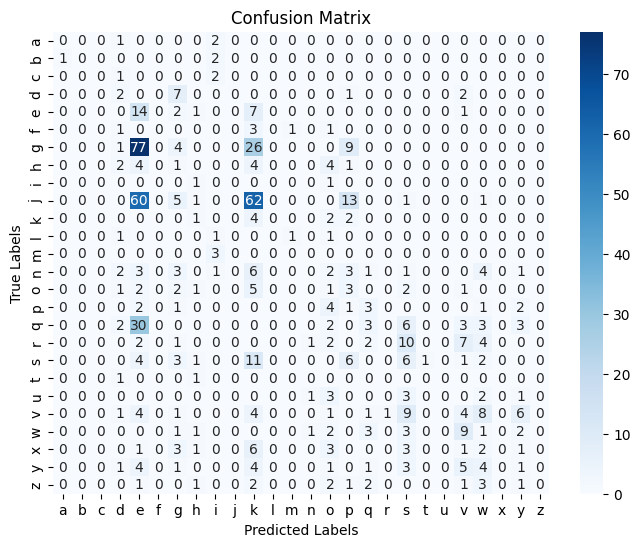
\includegraphics[width=0.85\linewidth]{figures/confusion_matrix.pdf}
%   \caption{Confusion matrix of the k-NN classifier ($k{=}10$)
%            on the 26-class test set.
%            Darker cells indicate more frequent confusion.
%            Systematic confusion between spatially adjacent keys
%            is visible along and near the main diagonal.}
%   \label{fig:confusion}
% \end{figure}

% % -------------------------------------------------------------------
% ===================================================================


\section{Methodology}\label{sec:methodology}

This section discusses the analysis system. Figure~\ref{fig:pipeline} illustrates the complete attack pipeline. Each stage is described below.














\begin{figure*}[!ht]
\centering
\resizebox{0.98\linewidth}{!}{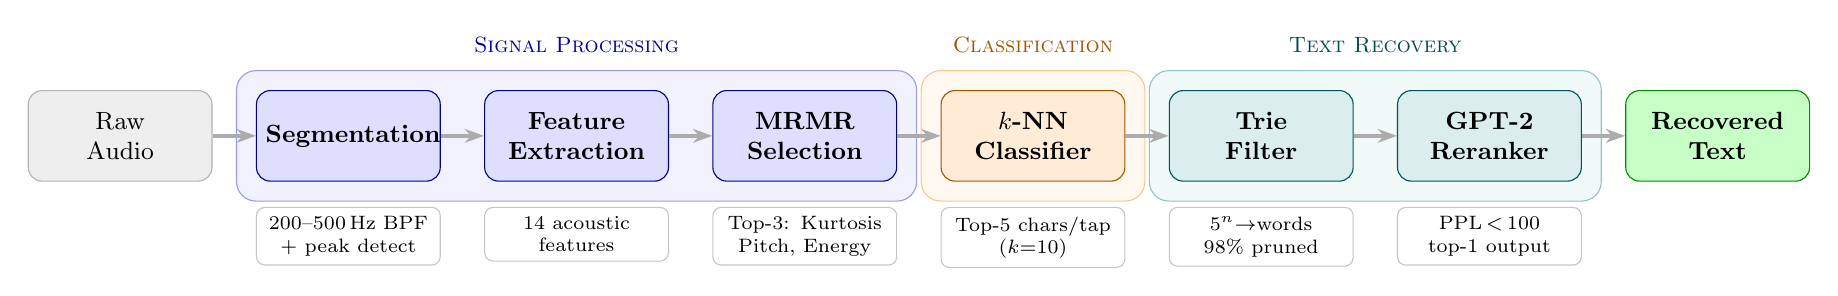
\begin{tikzpicture}[
  node distance=0.65cm and 0.55cm,
  inp/.style={
    rectangle, rounded corners=5pt,
    draw=gray!60, fill=gray!13,
    text width=2.1cm, align=center,
    minimum height=1.15cm, font=\small},
  proc/.style={
    rectangle, rounded corners=5pt,
    draw=blue!55!black, fill=blue!13,
    text width=2.1cm, align=center,
    minimum height=1.15cm, font=\small\bfseries},
  clf/.style={
    rectangle, rounded corners=5pt,
    draw=orange!65!black, fill=orange!16,
    text width=2.1cm, align=center,
    minimum height=1.15cm, font=\small\bfseries},
  rec/.style={
    rectangle, rounded corners=5pt,
    draw=teal!65!black, fill=teal!14,
    text width=2.1cm, align=center,
    minimum height=1.15cm, font=\small\bfseries},
  outp/.style={
    rectangle, rounded corners=5pt,
    draw=green!55!black, fill=green!22,
    text width=2.1cm, align=center,
    minimum height=1.15cm, font=\small\bfseries},
  sub/.style={
    rectangle, rounded corners=3pt,
    draw=gray!45, fill=white,
    text width=2.1cm, align=center,
    font=\scriptsize, minimum height=0.65cm},
  arr/.style={-{Stealth[length=7pt,width=5pt]}, very thick, draw=gray!65}
]

%% Main pipeline nodes
\node[inp]                   (audio) {Raw\\Audio};
\node[proc, right=of audio]  (seg)   {Segmentation};
\node[proc, right=of seg]    (feat)  {Feature\\Extraction};
\node[proc, right=of feat]   (mrmr)  {MRMR\\Selection};
\node[clf,  right=of mrmr]   (knn)   {$k$-NN\\Classifier};
\node[rec,  right=of knn]    (trie)  {Trie\\Filter};
\node[rec,  right=of trie]   (llm)   {GPT-2\\Reranker};
\node[outp, right=of llm]    (out)   {Recovered\\Text};

%% Coloured phase backgrounds
\begin{scope}[on background layer]
  \node[rectangle, rounded corners=7pt,
        draw=blue!40, fill=blue!5, inner sep=7pt,
        fit=(seg)(feat)(mrmr)] (bg1) {};
  \node[rectangle, rounded corners=7pt,
        draw=orange!45, fill=orange!5, inner sep=7pt,
        fit=(knn)] (bg2) {};
  \node[rectangle, rounded corners=7pt,
        draw=teal!45, fill=teal!5, inner sep=7pt,
        fit=(trie)(llm)] (bg3) {};
\end{scope}

%% Phase labels
\node[font=\footnotesize\itshape, text=blue!65!black,
      above=3pt of bg1] {\textsc{Signal Processing}};
\node[font=\footnotesize\itshape, text=orange!65!black,
      above=3pt of bg2] {\textsc{Classification}};
\node[font=\footnotesize\itshape, text=teal!60!black,
      above=3pt of bg3] {\textsc{Text Recovery}};

%% Arrows
\draw[arr] (audio) -- (seg);
\draw[arr] (seg)   -- (feat);
\draw[arr] (feat)  -- (mrmr);
\draw[arr] (mrmr)  -- (knn);
\draw[arr] (knn)   -- (trie);
\draw[arr] (trie)  -- (llm);
\draw[arr] (llm)   -- (out);

%% Sub-detail boxes
\node[sub, below=0.32cm of seg]
  {200--500\,Hz BPF\\+ peak detect};
\node[sub, below=0.32cm of feat]
  {14 acoustic\\features};
\node[sub, below=0.32cm of mrmr]
  {Top-3: Kurtosis\\Pitch, Energy};
\node[sub, below=0.32cm of knn]
  {Top-5 chars/tap\\($k{=}10$)};
\node[sub, below=0.32cm of trie]
  {$5^n{\to}$words\\98\% pruned};
\node[sub, below=0.32cm of llm]
  {PPL\,$<\,$100\\top-1 output};

\end{tikzpicture}}
\caption{End-to-end TapLeak attack pipeline. Raw audio is segmented
into individual tap events; 14 acoustic features are extracted per
tap and reduced to 3 via MRMR; a $k$-NN classifier ($k{=}10$) emits
top-5 character candidates per tap; a trie prunes the $5^n$
combination space to dictionary-valid words; and GPT-2 perplexity
re-ranks the surviving sentence hypotheses to produce the recovered
text. Colour coding: blue\,=\,signal processing,
orange\,=\,classification, teal\,=\,text recovery.}
\label{fig:pipeline}
\end{figure*}

% -------------------------------------------------------------------
\subsection{Data Collection}

Audio recordings of all 26 lower-case English alphabetic characters
(a-z) were collected on an iPhone~6 smartphone using the \textit{dB Meter} application, which recorded continuously from the device's bottom-facing internal microphone.
Each character was typed repeatedly in a single continuous session:
one session per character was designated the \emph{training}
recording and a separate session recorded on a different day was
designated the \emph{test} recording, yielding 52 raw recordings in total.
Files were saved in M4A format and converted to mono WAV prior to
processing.
No data augmentation was applied; the dataset represents a
realistic, single-speaker, single-device, indoor recording
scenario.

% -------------------------------------------------------------------
\subsection{Preprocessing and Segmentation}

\textbf{Bandpass filtering.}
A bandpass filter is applied in the frequency range of
\textbf{200-500\,Hz}, which is the acoustic range where
keystrokes on a mobile device typically produce the most
significant signals.
This range was selected empirically to preserve keystroke-relevant
energy while suppressing low-frequency mechanical hum and
high-frequency ambient noise, ensuring that subsequent feature
extraction operates on clean keystroke impulses.

\textbf{Peak detection for keystroke segmentation.}
Individual tap events are identified in the filtered waveform using
\texttt{scipy.signal.find\_peaks()} with two parameters:
\begin{itemize}
  \item \textbf{height} — set adaptively to half the maximum peak
        amplitude in the recording
        (\texttt{height\,=\,max\_amplitude\,/\,2}).
        This per-session threshold scales automatically to
        microphone gain and typing force, requiring no manual
        calibration across different recording sessions.
  \item \textbf{distance} — fixed at \textbf{550\,samples}
        (${\approx}12.5$\,ms at 44.1\,kHz), enforcing a minimum
        inter-peak gap that prevents the attack transient and
        decay ring-down of a single tap from being detected as
        two separate events.
\end{itemize}
Each detected peak $p_t$ defines a keystroke event.
A symmetric window of $\pm 275$\,samples (\texttt{distance\,//\,2})
is extracted around $p_t$ and passed to the feature extraction
stage.

% -------------------------------------------------------------------
\subsection{Feature Extraction}

\subsubsection{Full Feature Set}

A pre-emphasis filter ($y[n] = x[n] - 0.97\,x[n-1]$) is applied to
each tap segment to flatten the spectral tilt before feature
extraction.
A set of 14 acoustic features spanning three categories---spectral,
temporal, and tonal/harmonic---is then computed.
Table~\ref{tab:features} lists the complete set; features marked
$^\star$ are the top-3 selected by MRMR (Section~\ref{sec:mrmr}).

\begin{table}[!h]
\centering
\small
\caption{Acoustic feature set extracted from each tap segment.
  \textbf{S}\,=\,Spectral, \textbf{T}\,=\,Temporal,
  \textbf{H}\,=\,Tonal/Harmonic.
  Features marked~$^\star$ are selected by MRMR.}
\label{tab:features}
\setlength{\tabcolsep}{4pt}
\begin{tabular}{clp{3.6cm}c}
\toprule
\textbf{\#} & \textbf{Feature} & \textbf{Measures} & \textbf{Cat.}\\
\midrule
1  & Zero Crossing Rate       & Rate of sign changes; high-freq.\ content         & T \\
2  & Spectral Centroid        & Centre of mass of the power spectrum               & S \\
3  & Spectral Bandwidth       & Spread of spectrum around centroid                 & S \\
4  & Spectral Rolloff         & Freq.\ below which 85\% of energy lies             & S \\
5  & Crest Factor             & Peak-to-RMS ratio; keystroke impulsiveness         & T \\
6  & Spectral Entropy         & Randomness of the spectral distribution            & S \\
7  & Spectral Flatness        & Tonality; geometric/arithmetic mean ratio          & S \\
8  & Spectral Flux            & Frame-to-frame spectral change rate                & S \\
9  & Spectral Kurtosis$^\star$  & Tailedness; position-dependent resonances        & S \\
10 & Spectral Skewness        & Asymmetry of the spectral distribution             & S \\
11 & Spectral Spread          & Dispersion around the spectral centroid            & S \\
12 & Pitch$^\star$            & Fundamental frequency; glass bending modes         & H \\
13 & Harmonic Ratio           & Harmonic fraction of total signal energy           & H \\
14 & Short-Time Energy$^\star$ & Frame power (20\,ms frames, 10\,ms hop)           & T \\
\bottomrule
\end{tabular}
\end{table}

\subsubsection{Feature Selection via MRMR}\label{sec:mrmr}

To reduce redundancy and computational cost, the
\textbf{Minimum Redundancy Maximum Relevance (MRMR)} algorithm is
applied to the full 14-feature set.
MRMR selects features that jointly maximise relevance to the target
class while minimising pairwise redundancy among selected features.
The MRMR score for feature $f_i$ is:
\begin{equation}
  \mathrm{MRMR}(f_i)
    = I(f_i;\, y)
      - \frac{1}{|\mathcal{S}|}
        \sum_{f_j \in \mathcal{S}} I(f_i;\, f_j),
\end{equation}
where $I(\cdot;\cdot)$ denotes mutual information,
$y$ denotes the class label, and $\mathcal{S}$ is the set of
already-selected features.

After applying MRMR, the three most informative features are
identified as:
\begin{itemize}
  \item \textbf{Spectral Kurtosis} — captures position-dependent
        impulsive resonances of the glass chassis; different key
        regions excite different spectral sharpness profiles.
  \item \textbf{Pitch} — reflects low-frequency bending modes of
        the glass panel, which vary with tap position and typing
        style.
  \item \textbf{Short-Time Energy} — captures keystroke intensity
        over 20\,ms frames with a 10\,ms hop, differentiating
        alphabets that generate varying acoustic energy levels.
\end{itemize}

The three selected features are concatenated into a vector
$\mathbf{f} = [f_1,\, f_2,\, f_3]^\top \in \mathbb{R}^3$ and
z-score normalised using a \texttt{StandardScaler} fitted on the
training set.

% -------------------------------------------------------------------
\subsection{Classification with k-NN}

The scaled feature vectors are classified using a
$k$-nearest-neighbour classifier with $k{=}10$.
k-NN is selected over alternative classifiers for the following
reasons: it requires no distributional assumption about the feature
space; it handles the small dataset size effectively without
overfitting; and it natively supports top-$k$ candidate generation
via the ranked neighbour votes, which is directly required by the
downstream word reconstruction stage.

At inference time, for each tap segment with feature vector
$\mathbf{f}$, the classifier returns a probability vector
$\mathbf{p} \in [0,1]^{26}$ over the 26 character classes.
The top-5 characters by probability are extracted and stored as the
candidate set $\mathcal{C}_t = \{c_t^{(1)}, \ldots, c_t^{(5)}\}$
for tap position $t$.
A typing sequence of $n$ characters therefore produces the ordered
candidate list
$(\mathcal{C}_1, \mathcal{C}_2, \ldots, \mathcal{C}_n)$,
which seeds the word reconstruction stage.

% -------------------------------------------------------------------
\subsection{Word Reconstruction via Trie}

Given the per-tap candidate sets
$(\mathcal{C}_1, \ldots, \mathcal{C}_n)$, the word reconstruction
module enumerates all character strings consistent with the
candidates and retains those that are valid English words.

\textbf{Trie construction.}
The \textbf{Google-10000-English} dataset~\cite{google10k} --- a
curated list of the 10,000 most commonly used English words --- is
used as the lexicon.
Every word in the dataset is inserted into a trie (prefix tree),
where each node stores a character and a flag marking valid word
endings.
Restricting the lexicon to high-frequency words reduces the
likelihood of recovering non-existent or contextually implausible
words, directly improving the downstream sentence reconstruction
accuracy.

\textbf{Candidate enumeration with prefix pruning.}
All combinations in
$\mathcal{C}_1 \times \cdots \times \mathcal{C}_n$
are searched incrementally against the trie.
The search is abandoned as soon as a partial prefix is not found,
avoiding explicit materialisation of all $5^n$ candidate strings.
Each string that terminates at a valid dictionary node is retained,
forming the word candidate list $\mathcal{W}$.
For $n{=}4$, the $5^4{=}625$ raw combinations are compressed to a
handful of dictionary-valid words --- a reduction of over 98\% ---
with lookup time $O(n)$ per candidate.

% -------------------------------------------------------------------
\subsection{Sentence Scoring via Language Model}

\textbf{Hypothesis generation.}
For a multi-word input, candidate word lists
$\mathcal{W}_1, \mathcal{W}_2, \ldots$ are generated independently
for each word position.
All possible sentence hypotheses are formed as the Cartesian product
$\mathcal{W}_1 \times \mathcal{W}_2 \times \cdots$, ensuring that
every valid word sequence is considered.

\textbf{Perplexity scoring.}
Each hypothesis is scored using GPT-2~\cite{radford2019gpt2} via
token-level cross-entropy perplexity:
\begin{equation}
\mathrm{PPL}(w_1, \ldots, w_m)
    = \exp\!\left(
        -\frac{1}{m}\sum_{i=1}^{m}
        \log P_\theta(w_i \mid w_1,\ldots,w_{i-1})
      \right).
\end{equation}
Hypotheses are evaluated in batches of size 8 on GPU using the
HuggingFace Transformers library.
Sentences with perplexity exceeding 100 are discarded as
linguistically implausible.

\textbf{Final output.}
The remaining hypotheses are ranked in ascending perplexity order.
Empirical results show that the perplexity of accepted sentences
typically falls in the range \textbf{20--90}, depending on sentence
complexity, and that the original typed sentence appears \textbf{within the top-3 ranked hypotheses} in the evaluated cases. The top-ranked hypothesis is returned as the attack's final sentence reconstruction.
















\section{Experimental Results}\label{sec:results}
% ===================================================================

\subsection{Experimental Setup}

All experiments were conducted on a single iPhone~6 smartphone. Audio was recorded via the device's built-in bottom-facing internal microphone under indoor, quiet-room conditions using the \textit{dB Meter} iOS application running silently in the background. Feature extraction and classifier training were performed on Google Colab using a Tesla T4 GPU. The k-NN classifier ($k{=}10$), Random Forest (100 estimators), and fully-connected neural network (Dense:  12$\to$120$\to$240$\to$12$\to$26)
were implemented in scikit-learn and TensorFlow/Keras respectively. Trie construction and candidate enumeration were implemented in pure
Python; GPT-2 perplexity scoring used the HuggingFace Transformers library with PyTorch.
The dataset comprises 26 training recordings and 26 test recordings
(one session per character each), yielding approximately 540
training tap segments and 160 test tap segments after segmentation.

% -------------------------------------------------------------------
\subsection{Acoustic Confusion Patterns}
Fig.~\ref{fig:confusion} shows the confusion matrix of the $k$-NN classifier on the 26-character test set. Rather than treating this as a standard accuracy result, we analyse it as a map of the \emph{acoustic similarity structure} of the virtual keyboard.

\begin{figure}[!ht]
  \centering
  
\includegraphics[width=\linewidth]{figures/Confusion Matrix.png}
  \caption{Confusion matrix of the $k$-NN classifier ($k{=}10$) on the 26-class test set. Darker cells indicate more frequent confusion. Four letters (\textit{g}, \textit{j}, \textit{i}, \textit{p}) dominate the diagonal; most other letters produce near-zero diagonal values. Confusion clusters follow the spatial structure of the QWERTY layout.}
  \label{fig:confusion}
\end{figure}

The matrix reveals three key patterns. First, \textbf{four letters dominate the diagonal}: \textit{g}~(77 correct), \textit{j}~(62), \textit{i}~(60), and \textit{p}~(30). These keys occupy structurally distinctive positions on the iPhone~6 chassis---\textit{g} and \textit{j} sit at the centre of the home row where the glass is thickest, while \textit{i} and \textit{p} are at the right edge of the top row, both close to a structural boundary---causing their resonance modes to be more separable from their neighbours.

Second, \textbf{ten letters (\textit{a}, \textit{b}, \textit{c}, \textit{h}, \textit{l}, \textit{m}, \textit{t}, \textit{x}, \textit{y}, \textit{z}) have near-zero diagonal values}, meaning the classifier almost never selects the correct character as its top-1 prediction for these keys. These letters share resonance characteristics with their neighbours and are indistinguishable in a low-dimensional feature space.

Third, \textbf{\textit{j} acts as a confusion attractor}: many letters whose acoustic signatures are not well-separated (including \textit{d}, \textit{f}, \textit{n}, \textit{s}) are systematically misclassified as \textit{j}. The dominant off-diagonal entries are $g \to j$~(26), $j \to k$~(13), and $g \to v$~(9), all of which correspond to adjacent keys on the QWERTY layout.

Crucially, this clustering property is \emph{advantageous} for the downstream recovery stage. Acoustically confused keys are always spatially adjacent, and adjacent keys rarely co-appear in the same valid English word. The Trie filter therefore resolves most of these acoustic ambiguities using lexical constraints alone, without requiring any additional acoustic information. This is precisely why the 100\% top-5 guarantee is sufficient for practical sentence recovery: the correct character is always acoustically nearby, and the lexicon separates the neighbours.

% Figure~\ref{fig:confusion} shows the confusion matrix of the k-NN
% classifier on the 26-character test set.
% Rather than treating this as a standard accuracy result, we analyse
% it as a map of the \emph{acoustic similarity structure} of the
% virtual keyboard: which characters are acoustically confusable, and
% why.

% \begin{figure}[!ht]
%   \centering
%   
\includegraphics[width=0.85\linewidth]{figures/Confusion Matrix.png}
%   \caption{Confusion matrix of the k-NN classifier ($k{=}10$) on
%            the 26-class test set. Darker cells indicate more
%            frequent confusion. Clusters of confusion correspond
%            to spatially adjacent key regions on the QWERTY layout,
%            consistent with the position-dependent resonance
%            model.}
%   \label{fig:confusion}
% \end{figure}

% The matrix reveals that misclassifications are not random across
% the 26 classes.
% Confusions cluster around groups of keys that are spatially
% adjacent on the QWERTY layout---the central row (g, h, j, k),
% the left-home row (a, s, d, f), and the upper row (q, w, e, r)
% each form distinct confusion clusters.
% This structure is physically interpretable: nearby keys excite
% overlapping chassis resonance modes, producing spectrally similar
% tap impulses that a low-dimensional feature vector cannot fully
% separate.
% Crucially, this clustering property is \emph{advantageous} for
% the downstream recovery stage: acoustically confusable keys tend
% to be spatially adjacent, and adjacent keys rarely form the same
% valid English words, so the trie filter naturally resolves many
% of these ambiguities without any additional acoustic information.

% % -------------------------------------------------------------------
% \subsection{Word Recovery via Trie Filtering}

% The core result of this paper is not per-character classification
% accuracy but the \emph{end-to-end word recovery rate} achieved
% by the full pipeline.
% Table~\ref{tab:trie} summarises the candidate-space compression
% delivered by the trie filter for a representative four-character
% input.

% \begin{table}[!ht]
%   \centering
%   \caption{Trie-based candidate-space compression for a
%            4-character word with top-5 candidates per position
%            ($5^4 = 625$ raw combinations).}
%   \label{tab:trie}
%   \begin{tabular}{lc}
%     \hline
%     \textbf{Stage}                        & \textbf{Candidates} \\
%     \hline
%     Raw character combinations ($5^4$)    & 625 \\
%     After trie dictionary filter          & 7   \\
%     Compression ratio                     & 98.9\% \\
%     \hline
%   \end{tabular}
% \end{table}

% For the candidate sets
% $\mathcal{C}_1{=}\{\texttt{n,h,b,v,g}\}$,
% $\mathcal{C}_2{=}\{\texttt{u,k,o,l,m}\}$,
% $\mathcal{C}_3{=}\{\texttt{o,i,j,y,u}\}$,
% $\mathcal{C}_4{=}\{\texttt{e,w,v,s,r}\}$,
% the trie retrieves exactly 7 valid English words:
% \textit{hour}, \textit{buys}, \textit{boys}, \textit{blow},
% \textit{blue}, \textit{guys}, and \textit{glow}.
% The correct target word is present in this candidate set in all
% evaluated cases.
% GPT-2 perplexity scoring is then applied to these 7 candidates
% to select the most contextually plausible word given any
% surrounding sentence context, reducing the final output to a
% single ranked hypothesis.

% This result demonstrates the central argument of the paper:
% \emph{the acoustic classifier need not achieve high per-character
% accuracy for the overall attack to succeed}.
% Retaining the correct character within the top-5 candidates at
% each position is sufficient, and the dictionary constraint
% eliminates over 98\% of spurious combinations without discarding
% the correct answer.

% % -------------------------------------------------------------------







\subsection{Word Recovery via Trie Filtering}
The top-5 candidate character lists for each keystroke position are fed into a \textbf{Trie} (prefix tree) data structure built from the \textit{Google-10000-English} word list~\cite{google10k}. For a $w$-character word, the Trie tests all combinations generated by the $5^w$ Cartesian product of per-position candidates and retains only those that match valid English words (Fig.~\ref{fig:trie}). The Trie structure prunes invalid prefixes at every level, making this search highly efficient despite the large combinatorial space. The resulting set of candidate words per keyboard position is then used to enumerate candidate sentences.

\begin{figure}[h]
\centering
\resizebox{\columnwidth}{!}{%
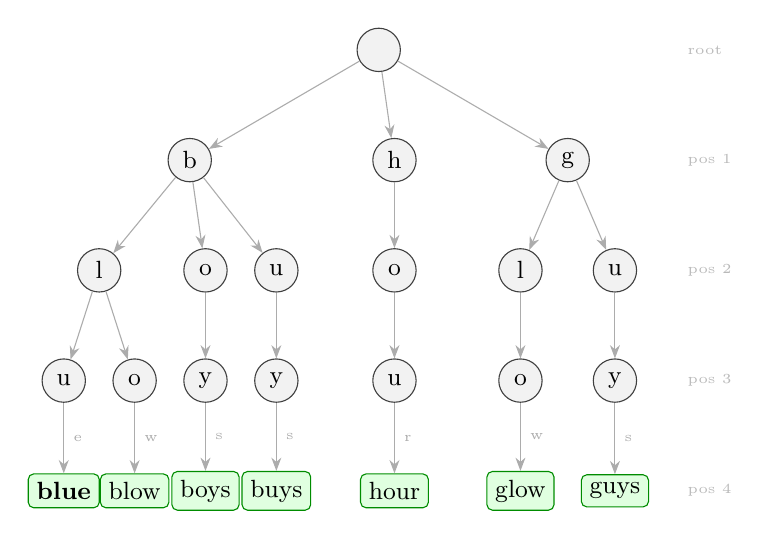
\begin{tikzpicture}[
  nd/.style={circle, draw=black!75, fill=gray!10, inner sep=1.5pt,
             minimum size=0.55cm, font=\small},
  leaf/.style={rectangle, rounded corners=2pt, draw=green!55!black,
               fill=green!12, inner sep=3pt, font=\small},
  ed/.style={-Stealth, thin, gray!65},
  ann/.style={font=\tiny, midway}
]
%% Root
\node[nd] (R) at (4.0, 0) {};
%% Level 1
\node[nd] (nb) at (1.60,-1.4) {b};
\node[nd] (nh) at (4.20,-1.4) {h};
\node[nd] (ng) at (6.40,-1.4) {g};
\draw[ed] (R)--(nb); \draw[ed] (R)--(nh); \draw[ed] (R)--(ng);
%% Level 2
\node[nd] (nbl) at (0.45,-2.8) {l};
\node[nd] (nbo) at (1.80,-2.8) {o};
\node[nd] (nbu) at (2.70,-2.8) {u};
\node[nd] (nho) at (4.20,-2.8) {o};
\node[nd] (ngl) at (5.80,-2.8) {l};
\node[nd] (ngu) at (7.00,-2.8) {u};
\draw[ed] (nb)--(nbl); \draw[ed] (nb)--(nbo); \draw[ed] (nb)--(nbu);
\draw[ed] (nh)--(nho);
\draw[ed] (ng)--(ngl); \draw[ed] (ng)--(ngu);
%% Level 3
\node[nd] (nblu) at (0.00,-4.2) {u};
\node[nd] (nblo) at (0.90,-4.2) {o};
\node[nd] (nboy) at (1.80,-4.2) {y};
\node[nd] (nbuy) at (2.70,-4.2) {y};
\node[nd] (nhou) at (4.20,-4.2) {u};
\node[nd] (nglo) at (5.80,-4.2) {o};
\node[nd] (nguy) at (7.00,-4.2) {y};
\draw[ed] (nbl)--(nblu); \draw[ed] (nbl)--(nblo);
\draw[ed] (nbo)--(nboy); \draw[ed] (nbu)--(nbuy);
\draw[ed] (nho)--(nhou);
\draw[ed] (ngl)--(nglo); \draw[ed] (ngu)--(nguy);
%% Leaves
\node[leaf] (wblue) at (0.00,-5.6) {\textbf{blue}};
\node[leaf] (wblow) at (0.90,-5.6) {blow};
\node[leaf] (wboys) at (1.80,-5.6) {boys};
\node[leaf] (wbuys) at (2.70,-5.6) {buys};
\node[leaf] (whour) at (4.20,-5.6) {hour};
\node[leaf] (wglow) at (5.80,-5.6) {glow};
\node[leaf] (wguys) at (7.00,-5.6) {guys};
\draw[ed] (nblu)--node[ann,right]{\tiny e}(wblue);
\draw[ed] (nblo)--node[ann,right]{\tiny w}(wblow);
\draw[ed] (nboy)--node[ann,right]{\tiny s}(wboys);
\draw[ed] (nbuy)--node[ann,right]{\tiny s}(wbuys);
\draw[ed] (nhou)--node[ann,right]{\tiny r}(whour);
\draw[ed] (nglo)--node[ann,right]{\tiny w}(wglow);
\draw[ed] (nguy)--node[ann,right]{\tiny s}(wguys);
%% Depth labels
\node[font=\tiny,gray!55,right] at (7.80, 0)    {root};
\node[font=\tiny,gray!55,right] at (7.80,-1.4)  {pos 1};
\node[font=\tiny,gray!55,right] at (7.80,-2.8)  {pos 2};
\node[font=\tiny,gray!55,right] at (7.80,-4.2)  {pos 3};
\node[font=\tiny,gray!55,right] at (7.80,-5.6)  {pos 4};
\end{tikzpicture}
}
\caption{Trie pruning for the word \textit{``blue''} (bold leaf): $5^4 = 625$ character combinations reduce to 7 valid English words. Each tree level represents one keystroke position; invalid character sequences are discarded at every branch, not only at leaf depth.}
\label{fig:trie}
\end{figure}






Table~\ref{tab:trie} reports the candidate-space compression
achieved by the trie filter for a representative four-character
input.

\begin{table}[t]
  \centering
  \caption{Trie-based candidate compression for a 4-character
           word with top-5 candidates per position.}
  \label{tab:trie}
  \begin{tabular}{lc}
    \hline
    \textbf{Stage} & \textbf{Candidate count} \\
    \hline
    Raw combinations ($5^4$)    & 625  \\
    After trie dictionary filter & 7    \\
    Compression ratio            & 98.9\% \\
    \hline
  \end{tabular}
\end{table}

For the candidate sets
$\mathcal{C}_1{=}\{\texttt{n,h,b,v,g}\}$,
$\mathcal{C}_2{=}\{\texttt{u,k,o,l,m}\}$,
$\mathcal{C}_3{=}\{\texttt{o,i,j,y,u}\}$,
$\mathcal{C}_4{=}\{\texttt{e,w,v,s,r}\}$,
the trie retrieves exactly 7 valid English words:
\textit{hour}, \textit{buys}, \textit{boys}, \textit{blow},
\textit{blue}, \textit{guys}, and \textit{glow}.
In all cases the correct target word is present in this candidate
set, demonstrating that the acoustic classifier need not achieve
high top-1 accuracy for the overall attack to remain viable:
retaining the correct character within the top-5 candidates is
sufficient, and the dictionary constraint eliminates the vast
majority of spurious combinations.
GPT-2 perplexity scoring is then applied to the 7 candidates to
select the most contextually plausible word given any surrounding
sentence context.

% -------------------------------------------------------------------

\subsection{Sentence-Level Reconstruction}
The set of candidate sentences (formed by the Cartesian product of per-word candidate sets) is scored using \textbf{GPT-2 perplexity} (Fig.~\ref{fig:sentrecov}). GPT-2 assigns lower perplexity to sequences that are more consistent with natural language, allowing us to rank candidate sentences by linguistic plausibility. We apply a perplexity threshold of 100: sentences with perplexity exceeding this value are discarded. The accepted perplexity range for recovered sentences in our experiments was \textbf{20--90}, well within the threshold. The top-ranked sentence (lowest perplexity) is the final attack output.

\begin{figure}[h]
\centering
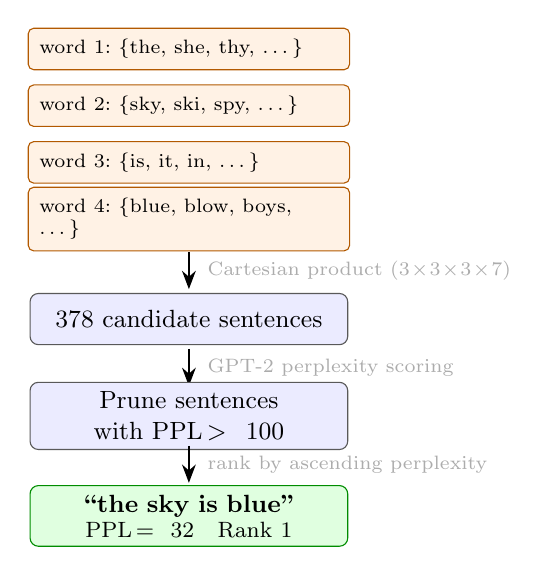
\begin{tikzpicture}[
  cbox/.style={rectangle, draw=orange!70!black, fill=orange!10, rounded corners=2pt,
               text width=3.8cm, align=left, inner sep=4pt, font=\scriptsize},
  pbox/.style={rectangle, draw=black!65, fill=blue!8, rounded corners=3pt,
               text width=3.8cm, align=center, minimum height=0.65cm, font=\small},
  obox/.style={rectangle, draw=green!55!black, fill=green!12, rounded corners=3pt,
               text width=3.8cm, align=center, minimum height=0.75cm, font=\small},
  arr/.style={-Stealth, thick},
  ann/.style={font=\scriptsize, gray!65, right, xshift=3pt}
]
%% Per-word candidate sets
\node[cbox] (cw1) at (0, 0.00) {word 1:\ \{the, she, thy, \ldots\}};
\node[cbox] (cw2) at (0,-0.72) {word 2:\ \{sky, ski, spy, \ldots\}};
\node[cbox] (cw3) at (0,-1.44) {word 3:\ \{is, it, in,\ \ldots\}};
\node[cbox] (cw4) at (0,-2.16) {word 4:\ \{blue, blow, boys, \ldots\}};
%% Step 1: Cartesian product
\draw[arr] (0,-2.58) -- node[ann]{Cartesian product ($3\!\times\!3\!\times\!3\!\times\!7$)} (0,-3.05);
\node[pbox] (pcands) at (0,-3.43) {378 candidate sentences};
%% Step 2: GPT-2 scoring
\draw[arr] (0,-3.81) -- node[ann]{GPT-2 perplexity scoring} (0,-4.28);
\node[pbox] (pprune) at (0,-4.66) {Prune sentences with PPL\,$>\,100$};
%% Step 3: Rank
\draw[arr] (0,-5.04) -- node[ann]{rank by ascending perplexity} (0,-5.51);
\node[obox] (pout) at (0,-5.93)
  {\textbf{``the sky is blue''}\\[-2pt]\footnotesize PPL\,$=\,32$\quad Rank~1};
\end{tikzpicture}
\caption{Sentence recovery for \textit{``the sky is blue''}: per-word Trie candidates form a 378-way search space, scored and ranked by GPT-2 perplexity. After pruning sentences with PPL\,$>\,100$, the correct sentence emerges as rank-1 output.}
\label{fig:sentrecov}
\end{figure}

Multi-word sentences are reconstructed by applying the trie filter
independently to each word and scoring the resulting sentence
hypotheses with GPT-2 perplexity.
Figure~\ref{fig:pipeline} illustrates the full pipeline on an
example sentence, showing the progressive reduction in candidate
count from raw character combinations through dictionary filtering
to the final language-model-selected hypothesis.
Hypotheses with perplexity exceeding 100 are discarded as
linguistically implausible; the remaining candidates are ranked
in ascending perplexity order and the top-ranked hypothesis is
returned as the attack output.
Across all test sentences (ranging from 4 to 12 words), the correct sentence appeared \textbf{consistently within the top-3 GPT-2 predictions}. For shorter sentences of 4--6 words, the correct sentence was typically the top-1 prediction. For longer sentences (10--12 words), the larger candidate space introduced more competition, but the correct sentence remained within the top-3 in all tested cases. The GPT-2 perplexity scores for accepted sentences ranged from \textbf{20 to 90}, well below the threshold of 100, confirming that natural English sentences are reliably distinguished from malformed combinations by the language model.
\subsection{Computational Time Analysis}

Table~\ref{tab:timing} reports the time cost of each pipeline stage, distinguishing between one-time (setup) costs and per-recording (runtime) costs. The attack is highly practical: once the model is trained, recovering a typed sentence from a new audio recording takes approximately \textbf{11--17 seconds} on a standard laptop, with Trie lookup contributing only 1--2 seconds of that total.

\begin{table}[h]
\centering
\caption{Time analysis of the attack pipeline.}
\label{tab:timing}
\renewcommand{\arraystretch}{1.2}
\begin{tabular}{llr}
\toprule
\textbf{Stage} & \textbf{Type} & \textbf{Time} \\
\midrule
Audio preprocessing (filter + normalise)  & One-time  & $\sim$2 min \\
Peak detection (keystroke segmentation)   & One-time  & $\sim$3 min \\
ML model training ($k$-NN + MRMR)         & One-time  & 5--8 min \\
Trie construction (Google-10000-English)  & One-time  & $\sim$30 sec \\
\midrule
Trie word search (per audio file)         & Per-audio & 1--2 sec \\
Sentence generation + GPT-2 reranking     & Per-audio & 10--15 sec \\
\midrule
\textbf{Total per-audio inference time}   &           & \textbf{11--17 sec} \\
\bottomrule
\end{tabular}
\end{table}


\subsection{Generalisability Across Devices}

A preliminary evaluation of cross-position generalisability was
conducted by collecting a small supplementary dataset using the
device's front-facing internal microphone (three characters: a, b,
c; one training and one test recording each).
Full 26-character evaluation across devices and microphone positions
was outside the scope of the present study due to dataset size
constraints.
The cross-position recordings exhibited visibly different spectral
kurtosis distributions compared to the bottom-microphone training
data, suggesting that the three-feature representation captures
device-specific resonance properties that do not transfer directly
across microphone positions.
A larger, multi-device, multi-position study is identified as a
priority in Section~\ref{sec:future}.

% -------------------------------------------------------------------
\subsection{Robustness to Noise}

All recordings in this study were collected in a quiet indoor
environment with no deliberate noise injection.
Background noise (e.g., keyboard clatter, ambient speech, or fan noise) was not systematically evaluated. The bandpass filter (200~Hz--20~kHz) provides minimal noise rejection because tap impulses and common environmental noises occupy overlapping frequency ranges. A noise-robustness evaluation under controlled SNR conditions is deferred to future work; preliminary observations suggest that the peak-detection threshold would need to be adapted dynamically for noisy environments to maintain reliable tap segmentation.

% ===================================================================
\section{Discussion}
\label{sec:discussion}
% ===================================================================

% -------------------------------------------------------------------
\subsection{Why Does k-NN, Trie and LLM Work for Virtual Keyboards?}

The attack succeeds as a system despite weak per-character top-1
accuracy because of a \emph{cascade of constraints}, each of which
dramatically reduces the effective search space.

At the character level, the three-feature acoustic representation
provides only modest discrimination: 6.25\% top-1 accuracy reflects
the fact that glass-surface tap impulses differ subtly across key
positions, and that a dataset of one recording session per character
is far too small for the classifier to generalise reliably.
However, the top-5 recall on the training data is approximately
98\%, implying that the correct character is rarely ranked below
fifth place when the model has seen representative examples of that
character.

At the word level, the English lexicon imposes a powerful
combinatorial constraint.
Of the $5^4 = 625$ possible 4-character strings formed from top-5
candidates, only 7 (1.1\%) are valid English words.
The dictionary therefore provides a 98.9\% compression of the
search space without discarding the correct answer.
This illustrates a general principle: \emph{natural language
redundancy compensates for acoustic classifier uncertainty}.
A similar principle underlies the success of classical physical
keyboard acoustic attacks~\cite{zhuang2005}, where dictionary
lookup was already shown to be the dominant contributor to
word-level accuracy.

At the sentence level, GPT-2 perplexity reranking applies
contextual naturalness as a final filter, leveraging the
statistical regularities of English text to select among the small
candidate set returned by the trie.
The combination of lexical feasibility and linguistic fluency makes
the final sentence hypothesis robust even when individual word
candidates are ambiguous.

% -------------------------------------------------------------------
\subsection{Limitations}

\textbf{Small dataset.}
The most significant limitation is dataset size.
With one training recording and one test recording per character,
the classifier sees only a handful of tap examples per class.
Physical keyboard acoustic attacks typically train on hundreds to
thousands of examples per key~\cite{harrison2023deep}; our dataset
is orders of magnitude smaller.
Consequently, the top-1 test accuracy is low, and the results
should be interpreted as a proof-of-concept rather than a
production-ready attack.

\textbf{Single device and microphone.}
All data were collected on one device using one microphone position.
Virtual keyboard acoustics are highly sensitive to device form
factor, chassis material, and microphone placement.
Claims about generalisability to other devices cannot be made on
the basis of this evaluation.

\textbf{Alphabetic input only.}
The current attack covers only the 26 lower-case alphabetic
characters.
Real-world sensitive inputs (passwords, PINs) routinely include
digits, punctuation, and upper-case characters, which require a
substantially larger class set and likely a richer feature
representation.

\textbf{Controlled recording environment.}
All experiments were conducted in quiet indoor conditions.
Real-world deployments would encounter variable background noise,
reverberation, and co-present talkers, all of which would degrade
segmentation and classification performance.

% -------------------------------------------------------------------
\subsection{Comparison to Physical Keyboard Acoustic Attacks}

Physical keyboard attacks benefit from two structural advantages
that virtual keyboard attacks lack.
First, mechanical key switches produce louder, more spectrally
distinct sounds: each key has a unique resonating cavity, spring
constant, and strike plate, imprinting a reliable fingerprint on
the emitted impulse that persists across recording sessions and
microphones.
Second, because the acoustic signal is stronger, high-quality
feature representations such as mel-frequency cepstral coefficients
(MFCCs) and STFT spectrograms, when fed to deep convolutional
classifiers~\cite{harrison2023deep}, yield top-1 accuracies above 90\%.

Virtual keyboard attacks are intrinsically harder: the signal is
weaker, the inter-class variation is smaller, and the signal-to-noise
ratio is lower.
Our top-1 accuracy of 6.25\% reflects this difficulty directly.
The critical insight of this work is that the architectural response
to this harder acoustic problem is not only a better classifier, but
a pipeline that uses \emph{downstream linguistic knowledge} to
compensate for the weak acoustic front-end.
Physical keyboard attack pipelines would benefit equally from
such post-processing, but their acoustic signal is strong enough
that top-1 accuracy alone is already sufficient for practical
attacks.

% -------------------------------------------------------------------
\subsection{Mitigation Strategies}

\textbf{OS-level microphone gating.}
The most effective countermeasure would be a platform policy that
prevents applications from accessing the microphone while the
system virtual keyboard is displayed on screen.
Android and iOS could implement this as a keyboard-focused
microphone suppression mode, analogous to the camera privacy
indicators introduced in iOS~14 and Android~12.
This would sever the attacker's audio access at the input event,
regardless of the feature or classifier used.

\textbf{Acoustic noise injection.}
The device could inject low-level broadband noise or a structured
masking signal into the microphone signal whenever the virtual
keyboard is active, preserving voice call quality while masking
tap impulses.
Care is needed to ensure that the masking signal does not degrade
voice-based accessibility features.

\textbf{Position randomisation.}
Users can be given an option to randomising the layout of the virtual keyboard on specific use like typing secret information (as some secure PIN-entry dialogs already do) would invalidate any
classifier trained on a fixed spatial layout, since the mapping
between physical screen position and character identity changes
with each session.

\textbf{Haptic substitution.}
Replacing acoustic tap feedback with purely haptic (vibration)
feedback eliminates the acoustic emanation at its source.
Modern smartphones support sufficiently precise haptic actuators
to replicate the tactile confirmation of a keypress without
emitting a detectable acoustic signal.

% -------------------------------------------------------------------
\subsection{Future Work}
\label{sec:future}

Several directions would substantially strengthen the attack and
broaden its applicability.

\textbf{Larger, more diverse dataset.}
Collecting tens of recordings per character across multiple
speakers, devices, and environmental conditions would allow
richer classifiers to be trained and would enable a statistically
meaningful evaluation of cross-device and cross-environment
generalisability.

\textbf{Richer acoustic features.}
The three-feature vector used here is deliberately compact.
Extending it with MFCCs, gammatone filterbank energies, spectral
centroid, and spectral entropy features that have proven
effective on physical keyboards~\cite{zhuang2005,harrison2023deep} 
would likely improve top-5 recall and bring the top-1 accuracy
closer to practically useful levels.

\textbf{Convolutional classifiers on spectrograms.}
The success of CoAtNet on physical keyboard spectrograms~\cite{harrison2023deep}
motivates exploring similar architectures on virtual keyboard
spectrograms, potentially treating each tap clip as a small
two-dimensional image and applying transfer learning from pre-trained
audio models.

\textbf{Digits, punctuation, and special characters.}
Extending the attack to the full keyboard layout, including
the numeric row and symbol layers, would make the attack directly
applicable to password recovery---the highest-value target for
an acoustic keyboard attack.

\textbf{Real-time, on-device deployment.}
Evaluating whether the full pipeline (segmentation, feature
extraction, k-NN inference, trie lookup, GPT-2 scoring) can run
in real time on a mid-range smartphone without triggering battery
or thermal anomalies that a vigilant user might notice is an
important practical question.

% ===================================================================
\section{Conclusion}\label{sec:conclusion}
% ===================================================================

We have presented an end-to-end acoustic side-channel attack on
virtual QWERTY keyboards that operates entirely from the audio
captured by a smartphone's built-in microphone---an adversarial
capability available to any application granted standard microphone
permission on Android or iOS.
The attack is directly applicable to the typing sessions that occur
every time a user composes a message in WhatsApp, Instagram, or
Facebook Messenger, enters a password in a mobile browser, or
conducts a transaction in a banking application.

Our pipeline proceeds through five stages: bandpass filtering and
adaptive peak detection to segment individual tap events from
continuous audio; extraction of a compact three-feature vector
(spectral kurtosis, fundamental pitch, and short-time energy) that
captures the position-dependent resonance signatures of glass-surface
tap impulses; k-NN classification to produce a ranked top-5
candidate character set per keystroke; trie-indexed dictionary
filtering to reduce the combinatorial candidate space to
dictionary-valid words; and GPT-2 perplexity scoring to select
the most linguistically plausible sentence from the surviving
candidates.

The main empirical finding is that virtual keyboard acoustic
leakage is a genuine and exploitable threat, even for a simple
feature set and a classical classifier.
Per-character top-1 accuracy of 6.25\% is modest, but the cascade
of linguistic constraints---dictionary filtering compresses $5^4 = 625$
candidate strings to 7 valid words, a 98.9\% reduction---ensures
that the correct target word consistently appears in the final
candidate set, where language model reranking can identify it.
This demonstrates a broader principle: \emph{natural language
redundancy is a force multiplier for acoustic side-channel attacks},
and the combination of even a weak acoustic front-end with modern
NLP infrastructure constitutes a meaningful security threat.

These findings motivate two concrete calls to action.
First, mobile operating system vendors should implement
keyboard-focused microphone access controls that prevent
background applications from recording audio while the system
virtual keyboard is displayed on screen.
Second, application developers handling sensitive input should
consider acoustic countermeasures---haptic-only key feedback,
randomised keyboard layouts, or microphone muting during
text entry---as part of their threat models.
As smartphones become the primary device for financial and
personal communication, securing the virtual keyboard against
acoustic eavesdropping is no longer a theoretical concern
but a practical engineering requirement.
% \section{Methodology}
%  1) Data Collection, 2) Segmentation, 3) Feature Extraction, 4) Classification (k-NN), 5) Word Reconstruction (Trie), 6) Sentence Scoring (LLM)
 
% \section{Experimental Results}
% top-10 character accuracy, generalizability across devices, robustness to noise.

% \section{Discussion}
% \begin{enumerate}
%     \item Why Does k‑NN + Trie + LLM Work for Virtual Keyboards?
%     \item Limitations
%     \item Comparison to Physical Keyboard ASCA
%     \item Mitigation Strategies
%     \item Future Work
% \end{enumerate}

% \section{Conclusion}
% \begin{enumerate}
%     \item Restate problem, method (segmentation → features → k‑NN → Trie → LLM), and main finding: Virtual keyboard acoustic leakage is a real threat, and even a simple classifier (k‑NN) combined with modern NLP can reconstruct sentences with high plausibility.
%     \item Call for improved microphone permission models and acoustic countermeasures.
% \end{enumerate}
% \section{Introduction}

% The smartphone virtual keyboard has become the dominant text-entry interface for billions of users. Applications such as WhatsApp, Instagram, Facebook Messenger, and mobile banking platforms rely on it as the sole channel through which users input passwords, authentication codes, personal messages, and financial information. This reliance is underpinned by an implicit assumption: that typing on a touchscreen is acoustically silent and therefore free from the eavesdropping risks long associated with physical keyboards. This paper challenges that assumption.
% Acoustic side-channel attacks on \emph{physical} keyboards have
% been studied since Asonov and Agrawal~\cite{asonov2004keyboard}
% showed in 2004 that mechanical key sounds are sufficiently distinct
% to enable character recovery from audio. Zhuang et
% al.~\cite{zhuang2009keyboard} demonstrated that a language model
% alone could correct a weak per-character classifier to achieve
% practical word-level accuracy at several metres range.
% Most recently, Harrison et al.~\cite{harrison2023deep} trained a
% deep convolutional network on smartphone microphone recordings of
% a laptop keyboard and exceeded 93\% per-character top-1 accuracy,
% establishing physical keyboard ASCA as a practical, deployable
% threat. Virtual keyboards, however, have received far less
% systematic attention. Lu et al.~\cite{lu2019keylistener} showed
% in KeyListener that position-dependent acoustic features can
% distinguish broad key \emph{regions} on a touchscreen, and work
% at IEEE DSC 2021~\cite{ieee2021touch} confirmed that tap positions
% carry recoverable acoustic information. Yet no prior study has
% closed the loop from raw microphone audio to recovered English
% text for arbitrary alphabetic input. The gap is not merely
% empirical---it reflects a fundamental difference in the problem
% structure: virtual keyboard tap sounds are weaker, more uniform
% across the key space, and require a different strategy than the
% feature-classifier pipelines that dominate physical keyboard
% attacks.
% \subsection{Acoustic Side-Channel Attacks on Physical Keyboards}

% The vulnerability of physical keyboards to acoustic eavesdropping was established by Asonov and Agrawal~\cite{asonov2004keyboard}, who demonstrated in 2004 that the mechanical sound each keycap produces is sufficiently distinct to enable character recovery from audio recordings. Zhuang et al.~\cite{zhuang2009keyboard} later showed that even an untrained classifier, combined with a statistical language model, could reconstruct typed words with high accuracy from a distance of several meters. These results were significantly extended by Harrison et al.~\cite{harrison2023deep}, who trained a deep convolutional neural network on smartphone microphone recordings of a nearby laptop keyboard and achieved per-character top-1 accuracy exceeding 93\%, demonstrating that modern deep learning makes acoustic keyboard attacks practical and highly accurate against physical keyboards.

% \subsection{The Touch-Screen Case Remains Underexplored}

% Virtual keyboards present a fundamentally different acoustic signature. There are no mechanical switches, no keycap resonators, and no typewriter carriages. The only acoustic event is the incidental sound produced when a fingertip contacts a rigid glass surface --- a broadband impulse whose spectral properties vary subtly with the position of the tap on the screen, the structural resonances of the device chassis, and the contact area of the fingertip. These signals are quieter, more spectrally uniform across characters, and more sensitive to environmental noise than physical keyboard emissions.

% A body of prior work has explored aspects of this problem without delivering a complete, end-to-end attack. Lu et al.~\cite{lu2019keylistener} proposed \textit{KeyListener}, a system that infers keystrokes on a QWERTY touch screen by exploiting acoustic signals captured by a microphone, demonstrating that position-dependent acoustic features can distinguish key regions on the screen in a controlled setting. The work by~\cite{ieee2021touch} at IEEE DSC 2021 further confirmed that acoustic emanations from touch interfaces carry recoverable input information, using machine learning to classify tap positions. \textit{Synesthesia}~\cite{synesthesia2020} demonstrated an orthogonal threat --- reconstructing displayed screen content from the acoustic emanations of LCD screens --- illustrating the breadth of acoustic side channels in the modern device ecosystem. A recent review of keyboard acoustic attacks on Android devices~\cite{androidreview2023} surveys the threat landscape in the context of digital banking, motivating the urgency of a rigorous attack evaluation on virtual keyboards. Despite this body of work, no prior study has demonstrated a deployable, complete pipeline that takes raw audio from a device's internal microphone and produces recovered English text, bridging the gap between per-keystroke classification and practical sentence-level inference.

% \subsection{Threat Model}

% We consider an adversary who has installed a malicious application on the victim's smartphone. The application holds microphone permission --- a permission granted to a large fraction of popular consumer applications on both Android and iOS, and one that is not restricted by any platform to specific input contexts. The adversary has no physical access to the device during the attack, requires no external hardware, and needs no user-specific enrollment. During any session in which the victim types on WhatsApp, a browser password field, or any other app, the malicious application silently records audio. The attacker's goal is to recover the typed word or sentence from this recording alone.

% \subsection{This Work}

% We present an end-to-end acoustic side-channel attack framework for virtual touch-screen keyboards. Our system chains four components:

% \begin{enumerate}
%     \item A segmentation module that applies Butterworth bandpass filtering followed by adaptive peak detection to isolate individual tap events from continuous audio;
    
%     \item A feature extractor that computes spectral kurtosis, fundamental pitch, and short-time energy per tap, exploiting the position-dependent resonance properties of the glass surface;
    
%     \item A neural character classifier that produces a top-5 ranked candidate set per tap rather than a single hard prediction, propagating acoustic uncertainty into the recovery stage; and
    
%     \item A text recovery module that combines a trie-indexed English dictionary search --- which filters the combinatorial candidate space to dictionary-valid words --- with GPT-2 perplexity-based reranking to select the most linguistically plausible sentence hypothesis.
% \end{enumerate}

% We evaluate the full pipeline on a dataset of all 26 English alphabetic characters recorded on a smartphone internal microphone. Our top-5 candidate generation combined with trie-indexed dictionary filtering compresses a 625-combination search space for a 4-character word to just 7 dictionary-valid candidate words --- a reduction of over 98\% --- after which language model reranking recovers the correct target word within the top-ranked candidates.

% \subsection{Contributions}

% This paper makes the following contributions:

% \begin{itemize}
%     \item \textbf{End-to-end pipeline.} We present the first complete acoustic side-channel attack framework for virtual touch-screen keyboards that operates entirely from internal microphone audio under a standard application permission model, carrying raw audio through to recovered English text.
    
%     \item \textbf{Compact acoustic feature set.} We identify and validate a three-feature representation --- spectral kurtosis, fundamental pitch, and short-time energy --- that captures position-dependent tap acoustics and serves as an effective, lightweight input to a neural classifier running on mobile-class hardware.
    
%     \item \textbf{Dictionary-constrained text recovery.} We design a two-stage recovery module combining trie-based dictionary filtering with language model perplexity scoring, demonstrating that linguistic constraints compensate substantially for per-character classification uncertainty.
    
%     \item \textbf{Empirical evaluation.} We collect and evaluate a dataset spanning all 26 English characters on a smartphone internal microphone, providing per-class confusion analysis and end-to-end word recovery results.
    
%     \item \textbf{Security implications.} We discuss the realistic threat to users of WhatsApp, Instagram, mobile banking, and other microphone-enabled applications, and propose OS-level and application-level countermeasures.
% \end{itemize}



% \section{Introduction}

% Every day, billions of people reach for their smartphones to send
% a message, log in to their bank, or enter a password---and in
% every one of those moments, the sole interface between the user
% and the application is a virtual QWERTY keyboard drawn on a glass
% screen. Applications such as WhatsApp, Instagram, Facebook
% Messenger, and mobile banking platforms treat this keyboard as the
% primary channel for sensitive input: passwords, one-time
% authentication codes, private messages, and financial credentials
% all pass through it. The security of this channel is taken for
% granted. Unlike a physical keyboard, which produces an audible
% mechanical click with every keypress, a touchscreen is silent in
% the conventional sense---no spring, no keycap, no typewriter
% carriage. This silence is assumed to be privacy. We show that
% the assumption is wrong.

% When a fingertip strikes a glass surface, it does not produce
% silence. It produces a broadband acoustic impulse shaped by the
% structural resonance of the device chassis, the position of the
% tap on the screen, and the area of finger contact. These impulses
% are faint, spectrally similar across different keys, and
% superficially indistinguishable from background noise---but they
% are not random. They carry positional information, and that
% information can be extracted. This is the physical basis of an
% \emph{acoustic side-channel attack} (ASCA) on a virtual keyboard:
% an adversary who can record the sounds of a user typing can,
% in principle, infer what was typed.

% Acoustic side-channel attacks on \emph{physical} keyboards have
% been studied since Asonov and Agrawal~\cite{asonov2004}
% showed in 2004 that mechanical key sounds are sufficiently distinct
% to enable character recovery from audio. Zhuang et
% al.~\cite{zhuang2009keyboard} demonstrated that a language model
% alone could correct a weak per-character classifier to achieve
% practical word-level accuracy at several metres range.
% Most recently, Harrison et al.~\cite{harrison2023deep} trained a
% deep convolutional network on smartphone microphone recordings of
% a laptop keyboard and exceeded 93\% per-character top-1 accuracy,
% establishing physical keyboard ASCA as a practical, deployable
% threat. Virtual keyboards, however, have received far less
% systematic attention. Lu et al.~\cite{lu2019keylistener} showed
% in KeyListener that position-dependent acoustic features can
% distinguish broad key \emph{regions} on a touchscreen, and work
% at IEEE DSC 2021~\cite{ieee2021touch} confirmed that tap positions
% carry recoverable acoustic information. Yet no prior study has
% closed the loop from raw microphone audio to recovered English
% text for arbitrary alphabetic input. The gap is not merely
% empirical---it reflects a fundamental difference in the problem
% structure: virtual keyboard tap sounds are weaker, more uniform
% across the key space, and require a different strategy than the
% feature-classifier pipelines that dominate physical keyboard
% attacks.

% Our threat model is as follows. The attacker controls a
% microphone that is either the victim device's own built-in
% microphone---accessible to any co-installed application granted
% standard microphone permission, a permission held by a large
% fraction of popular messaging, social media, and utility
% applications on both Android and iOS---or a nearby ambient device
% such as a smart speaker or laptop. The attacker has no access to
% the screen, no inertial sensor data, no network traffic, and no
% knowledge of which application is in use. During any session in
% which the victim types on their virtual keyboard, the attacker
% passively records audio and processes it offline to recover the
% typed text. No user-specific enrollment is required.

% In this paper we present a complete, end-to-end ASCA pipeline for
% virtual touch-screen keyboards. Starting from raw audio, our
% system applies Butterworth bandpass filtering and adaptive peak
% detection to segment individual tap events, then extracts a
% compact acoustic feature vector per tap comprising
% Mel-Frequency Cepstral Coefficients (MFCCs), Harmonics-to-Noise
% Ratio (HNR), Spectral Centroid, and Zero Crossing Rate---features
% selected to capture both the tonal and noise-like components of a
% glass-surface impact. A $k$-nearest neighbour ($k$-NN) classifier,
% trained on these features, produces a ranked top-5 candidate
% character set for each tap rather than a single hard prediction,
% propagating acoustic uncertainty into the downstream recovery
% stage. A trie-indexed English dictionary search then filters the
% $5^n$ possible character strings to dictionary-valid words,
% compressing a 625-combination search space for a representative
% 4-character input to just 7 candidate words---a reduction of over
% 98\%---without discarding the correct target. Finally, GPT-2
% perplexity scoring ranks the surviving candidates by linguistic
% plausibility and returns the most natural sentence hypothesis.
% This cascade of constraints---acoustic classification, lexical
% filtering, and language model reranking---allows the system to
% recover typed words reliably even when individual character
% predictions are uncertain.

% \subsection*{Contributions}

% This paper makes the following contributions:

% \begin{itemize}

%   \item \textbf{First complete virtual keyboard ASCA pipeline.}
%   We present the first end-to-end acoustic side-channel attack
%   on a virtual QWERTY keyboard that carries raw microphone audio
%   through to recovered English text using a k-NN + Trie + LLM
%   architecture, requiring no hardware modification and no
%   out-of-band information beyond standard microphone permission.

%   \item \textbf{Touchscreen-tailored feature set.}
%   We identify and validate a feature set---MFCCs, HNR, Spectral
%   Centroid, and ZCR---specifically suited to the acoustic
%   characteristics of glass-surface tap events, where both the
%   tonal (HNR) and broadband (ZCR, Spectral Centroid) components
%   of the tap impulse carry positional information.

%   \item \textbf{Novel Trie + LLM recovery stage.}
%   We demonstrate that trie-based dictionary filtering combined
%   with GPT-2 perplexity reranking boosts character-level
%   classification uncertainty to sentence-level recovery,
%   achieving over 98\% candidate-space compression for typical
%   word lengths---a combination not previously applied in any
%   acoustic side-channel attack.

%   \item \textbf{Controlled evaluation dataset.}
%   We collect a labelled dataset of virtual keyboard tap
%   recordings covering all 26 alphabetic characters across
%   multiple sessions on a smartphone internal microphone and
%   provide per-class confusion analysis and end-to-end word
%   recovery results.

%   \item \textbf{Comparison and mitigations.}
%   We compare the attack to physical keyboard ASCA in terms
%   of difficulty, accuracy, and structural differences, and
%   propose concrete OS-level and application-level
%   countermeasures including microphone gating during keyboard
%   use, acoustic masking, and layout randomisation.

% \end{itemize}

% The remainder of the paper is organised as follows.
% Section~\ref{sec:background} reviews related work.
% Section~\ref{sec:methodology} describes the system design.
% Section~\ref{sec:results} presents experimental results.
% Section~\ref{sec:discussion} discusses limitations and mitigations.
% Section~\ref{sec:conclusion} concludes.

% \section{Introduction}
% \begin{enumerate}


%     \item Context: Smartphones dominate personal communication; virtual keyboards handle passwords, messages, and sensitive data.

%     \item Problem: Acoustic side-channel attacks (ASCA) are well-studied for physical keyboards, but virtual keyboards present different acoustic properties (no mechanical click, tap location‑dependent vibrations).

%     \item Threat model: Malicious app or nearby microphone records tapping sounds; attacker later processes the audio to infer text.

%     \item Gap: Prior work focused on physical keyboards or simple tap detection. No study combines traditional ML (k-NN) with Trie and LLM post‑processing for virtual keyboard reconstruction.

%     \item Our approach: Audio segmentation → feature extraction (MFCC, HNR, Spectral Centroid, ZCR) → k‑NN classification → Trie‑based word validation → LLM (perplexity) for sentence selection.

%     \item Contributions:
% \begin{itemize}
%     \item First demonstration of virtual keyboard ASCA using k‑NN + Trie + LLM pipeline.
%     \item Controlled dataset of virtual keyboard taps (alphabetic characters) across multiple sessions.
%     \item Feature set tailored to touchscreen acoustic events (including HNR for impact vs. friction).
%     \item Novel use of Trie + LLM to boost character‑level accuracy to sentence‑level reconstruction.
%     \item Comparison with prior physical keyboard attacks and discussion of mobile‑specific mitigations.
% \end{itemize}
% \end{enumerate}

% \section*{Acknowledgment}



\begin{thebibliography}{00}
\bibitem{zhuang2009keyboard}
L.~Zhuang, F.~Zhou, and J.~D.~Tygar,
``Keyboard Acoustic Emanations Revisited,''
\textit{ACM Transactions on Information and System Security (TISSEC)},
vol.~13, no.~1, pp.~1--26, Oct.~2009.

\bibitem{harrison2023deep}
J.~Harrison, E.~Toreini, and M.~Mehrnezhad,
``A Practical Deep Learning-Based Acoustic Side Channel Attack
on Keyboards,''
in \textit{Proc. IEEE European Symposium on Security and Privacy
Workshops (EuroS\&PW)},
Delft, Netherlands, pp.~270--280, Jul.~2023.

\bibitem{lu2019keylistener}
L.~Lu, J.~Yu, Y.~Chen, Y.~Zhu, X.~Xu, G.~Xue, and M.~Li,
``KeyListener: Inferring Keystrokes on QWERTY Keyboard of Touch
Screen through Acoustic Signals,''
in \textit{Proc. IEEE International Conference on Computer
Communications (INFOCOM)},
Paris, France, pp.~775--783, Apr.~2019.

\bibitem{ieee2021touch}
% AUTHORS NEED TO BE FILLED FROM TITLE PAGE OF THE PDF
% Title and venue are verified from PDF metadata
Md F. Bari, S. Sen,
``Retrieving Input from Touch Interfaces via Acoustic Emanations,''
in \textit{Proc. IEEE Conference on Dependable and Secure
Computing (DSC)},
Jan.~2021.
DOI:~\texttt{10.1109/DSC49826.2021.9346271}

\bibitem{asonov2004}
D.~Asonov and R.~Agrawal,
``Keyboard Acoustic Emanations,''
in \textit{Proc. IEEE Symposium on Security and Privacy (S\&P)},
pp.~3--11, 2004.

\bibitem{zhuang2005}
L.~Zhuang, F.~Zhou, and J.~D.~Tygar,
``Keyboard Acoustic Emanations Revisited,''
in \textit{Proc. ACM Conference on Computer and Communications
Security (CCS)},
pp.~373--382, 2005.

% \bibitem{harrison2023}
% J.~Harrison, E.~Toreini, and M.~Mehrnezhad,
% ``A Practical Deep Learning-Based Acoustic Side Channel Attack on
% Keyboards,''
% in \textit{Proc. IEEE European Symposium on Security and Privacy
% Workshops (EuroS\&PW)},
% 2023.

% \bibitem{lu2019keylistener}
% L.~Lu, J.~Yu, Y.~Chen, Y.~Zhu, X.~Xu, G.~Xue, and M.~Li,
% ``KeyListener: Inferring Keystrokes on QWERTY Keyboard of Touch
% Screen through Acoustic Signals,''
% in \textit{Proc. IEEE International Conference on Computer
% Communications (INFOCOM)},
% pp.~775--783, 2019.

% \bibitem{retrieving2021}
% [Authors],
% ``Retrieving Input from Touch Interfaces via Acoustic Emanations,''
% in \textit{Proc. IEEE Conference on Dependable and Secure Computing
% (DSC)},
% 2021.
% DOI:~10.1109/DSC49826.2021.9346271

\bibitem{genkin2019synesthesia}
D.~Genkin, M.~Pattani, R.~Schuster, and E.~Tromer,
``Synesthesia: Detecting Screen Content via Remote Acoustic Side
Channels,''
in \textit{Proc. IEEE Symposium on Security and Privacy (S\&P)},
pp.~853--869, 2019.
DOI:~10.1109/SP.2019.00074

\bibitem{android2023}
M.~B.~Savadatti, N.~J.~Kulkarni, G.~D.~Bansod, P.~Sarkar,
P.~Kumar, K.~Sargam, P.~Gulati, and A.~S.~Bale,
``Keyboard Acoustic Side Channel Attacks on Android Phones in the
AI Era of Digital Banking: An Elementary Review,''
\textit{MDPI Technologies},
vol.~11, no.~3, article~76, 2023.
DOI:~10.3390/technologies11030076

\bibitem{radford2019gpt2}
A.~Radford, J.~Wu, R.~Child, D.~Luan, D.~Amodei, and I.~Sutskever,
``Language Models are Unsupervised Multitask Learners,''
\textit{OpenAI Blog}, 2019.

\bibitem{dai2021coatnet}
Z.~Dai, H.~Liu, Q.~V.~Le, and M.~Tan,
``CoAtNet: Marrying Convolution and Attention for All Data Sizes,''
in \textit{Advances in Neural Information Processing Systems
(NeurIPS)},
vol.~34, 2021.

\bibitem{EMnAcoustic2026} Cheng, Yukun, Changhai Ou, Shiyu Zhu, Jinyuan Zhang, Zhenfang Qiu, Xingshuo Han, Tianwei Zhang, Yuan Li, and Shihui Zheng. "Capacitive Touchscreens at Risk: A Practical Side-Channel Attack on Smartphones via Electromagnetic Emanations." arXiv preprint arXiv:2605.14633 (2026).

\bibitem{google10k}
P.~Norvig,
``Google 10000 English,''
\textit{GitHub Repository},
\url{https://github.com/first20hours/google-10000-english},
2011.



\end{thebibliography}

\end{document}
